\documentclass[final,review]{elsarticle}

\usepackage{lineno,hyperref}
\modulolinenumbers[5]

%%%%%%%%%%%%%%%%%%%%%%%%%%%%%%%%%%%%%%%%%%%%%%%%%%%%%%%%%%
\usepackage{graphicx}
\graphicspath{{./}}
\usepackage{algorithm}
\usepackage{algorithmic}
\usepackage{textcomp}
%%%%%%%%%%%%%%%%%%%%%%%%%%%%%%%%%%%%%%%%%%%%%%%%%%%%%%%%%%
\usepackage{booktabs}
\usepackage{longtable}
\usepackage[smaller]{acronym}
\usepackage{amsmath}
\usepackage{nicefrac}
\usepackage{xspace}
\usepackage{rotating}
\usepackage{url}
%\usepackage{ulem}

\newcommand{\ver}[1]{\textcolor{orange}{#1}}


\newcommand*{\eg}{e.g.\@\xspace}
\newcommand*{\ie}{i.e.\@\xspace}
\newcommand{\FL}[1]{\textsc{fl#1}}
\newcommand{\PELT}{\textsc{pelt}}
\newcommand{\DBSCAN}{\textsc{dbscan}}
%%%%%%%%%%%%%%%%%%%%%%%%%%%%%%%%%%%%%%%%%%%%%%%%%%%%%%%%%%
\usepackage{xcolor}
\definecolor{ams}{rgb}{1.0, 0.714, 0.467}
\definecolor{lhr}{rgb}{0.427, 0.714, 1.0}
\definecolor{stn}{rgb}{0.859, 0.82, 0.0}
\definecolor{ath}{rgb}{0.0, 0.427, 0.859}
\definecolor{mad}{rgb}{0.573, 0.0, 0.0}
\definecolor{lgw}{rgb}{0.0, 0.286, 0.286}
\definecolor{fco}{rgb}{0.141, 1.0, 0.141}
\definecolor{fra}{rgb}{0.286, 0.0, 0.573}
\definecolor{ltn}{rgb}{0.714, 0.859, 1.0}
\definecolor{cgd}{rgb}{0.573, 0.286, 0.0}

\newcommand{\airp}[1]{\textcolor{#1}{\textsc{#1}}}
%%%%%%%%%%%%%%%%%%%%%%%%%%%%%%%%%%%%%%%%%%%%%%%%%%%%%%%%%%
\newdefinition{rmk}{Remark}
\newdefinition{kpt}{Key Point}
%%%%%%%%%%%%%%%%%%%%%%%%%%%%%%%%%%%%%%%%%%%%%%%%%%%%%%%%%%
% Acronyms
\acrodef{FL}{Flight Level}
\acrodef{NM}{Nautical Miles}
\acrodef{TS}{Time Series}
\acrodef{ACC}{Area Control Centre}
\acrodef{ACF}{Autocorrelation function}
\acrodef{AIC}{Akaike Information Criterion}
\acrodef{ATM}{Air Traffic Management}
\acrodef{CCF}{Crosscorrelation function}
\acrodef{CDF}{Cumulative Distribution Function}
\acrodef{DDR}{Demand Data Repository}
\acrodef{ETA}{Expected Time of Arrival}
\acrodef{HDR}{High Density Rule}
\acrodef{MAE}{Mean Absolute Error}
\acrodef{MLE}{Maximum Likelihood Estimator}
\acrodef{MSE}{Mean Squared Error}
\acrodef{IID}{Independent Identically Distributed}
\acrodef{PDF}{Prob\-a\-bil\-i\-ty Density Function}
\acrodef{PMF}{Prob\-a\-bil\-i\-ty Mass Function}
\acrodef{TCC}{Terminal Control Centre}
\acrodef{UTC}{Coordinated Universal Time}
\acrodef{ASMA}{Arrival Sequencing and Metering Area}
\acrodef{ECAC}{European Civil Aviation Conference}
\acrodef{IATA}{International Air Transport Association}
\acrodef{ICAO}{International Civil Aviation Organization}
\acrodef{MBIC}{Modified Bayesian Information Criterion}
\acrodef{PSRA}{Pre-Scheduled Random Arrivals}
%%%%%%%%%%%%%%%%%%%%%%%%%%%%%%%%%%%%%%%%%%%%%%%%%%%%%%%%%%
\usepackage[T1]{fontenc}
% \usepackage{hyperref}
\usepackage{xr}
% Enable xr on overleaf
\makeatletter
\newcommand*{\addFileDependency}[1]{% argument=file name and extension
  \typeout{(#1)}
  \@addtofilelist{#1}
  \IfFileExists{#1}{}{\typeout{No file #1.}}
}
\makeatother

\newcommand*{\myexternaldocument}[1]{%
    \externaldocument{#1}%
    \addFileDependency{#1.tex}%
    \addFileDependency{#1.aux}%
}
\externaldocument[A-]{LL-A}
%%%%%%%%%%%%%%%%%%%%%%%%%%%%%%%%%%%%%%%%%%%%%%%%%%%%%%%%%%
\usepackage{hyperref}
%%%%%%%%%%%%%%%%%%%%%%%%%%%%%%%%%%%%%%%%%%%%%%%%%%%%%%%%%%



\journal{European Journal of Operational Research}

%%%%%%%%%%%%%%%%%%%%%%%
%% Elsevier bibliography styles
%%%%%%%%%%%%%%%%%%%%%%%
%% To change the style, put a % in front of the second line of the current style and
%% remove the % from the second line of the style you would like to use.
%%%%%%%%%%%%%%%%%%%%%%%

%% Numbered
%\bibliographystyle{model1-num-names}

%% Numbered without titles
%\bibliographystyle{model1a-num-names}

%% Harvard
%\bibliographystyle{model2-names.bst}\biboptions{authoryear}

%% Vancouver numbered
%\usepackage{numcompress}\bibliographystyle{model3-num-names}

%% Vancouver name/year
%\usepackage{numcompress}\bibliographystyle{model4-names}\biboptions{authoryear}

%% APA style
\bibliographystyle{model5-names}\biboptions{authoryear}

%% AMA style
%\usepackage{numcompress}\bibliographystyle{model6-num-names}

%% `Elsevier LaTeX' style
% \bibliographystyle{elsarticle-num}
%%%%%%%%%%%%%%%%%%%%%%%

\begin{document}

\begin{frontmatter}

\title{Predictive modeling of inbound demand at major European airports with Poisson and Pre-Scheduled Random Arrivals}
% \tnotetext[mytitlenote]{Fully documented templates are available in the elsarticle package on \href{http://www.ctan.org/tex-archive/macros/latex/contrib/elsarticle}{CTAN}.}

\author[address_cl]{Carlo Lancia\corref{corrauth}}
\cortext[corrauth]{Corresponding author.}
\ead{c.lancia@math.leidenuniv.nl}
\ead[url]{https://sites.google.com/view/clancia}

\author[address_gl]{Guglielmo Lulli}
\ead{g.lulli@lancaster.ac.uk}

\address[address_cl]{Leiden University Mathematical Institute, Niels Bohrweg 1, 2333 CA, Leiden, NL}
\address[address_gl]{Lancaster University Management School, Bailrigg, Lancaster, LA1 4YX, UK}

\begin{abstract}
  This paper presents an exhaustive study on the arrivals process at eight major European airports. Using inbound traffic data, we define, compare, and contrast a data-driven in-homogeneous Poisson and \ac{PSRA} point process on their ability to predict future demand.
%   Although, there is sufficient evidence that the inter-arrivals might follow an exponential distribution, this finding does not directly translate to evidence that the arrivals stream is Poisson.
%   The main reason is that finite-capacity constraints impose a correlation structure to the arrivals stream, which a Poisson model cannot capture.
As part of this analysis, we show both weaknesses and difficulties of using a non-homogeneous Poisson process to model with good approximation the arrivals stream. On the other hand, our novel and simple data-driven \ac{PSRA} model, captures and predicts with higher accuracy the main properties of the typical arrivals stream.
These results have important implication on modeling and simulation-based analyses of the inbound traffic aiming to improve the use of available capacity thus reducing air traffic delays. In a nutshell, the results lead to the conclusion that, in the European context, the \ac{PSRA} provides more accurate predictions.
\end{abstract}


\begin{keyword}
Transportation \sep Air traffic \sep Demand prediction \sep Data-driven modeling
\MSC[2010] 90B06 \sep  62P30
\end{keyword}

\end{frontmatter}

% \linenumbers

\section{Introduction}
\label{sec:introduction}

Air congestion is a regular and persistent phenomenon in the air traffic system in both the US and Europe.
Over the years, air traffic demand increased at a much faster pace compared to the increment of air-traffic-system capacity.
In the last decade, we have witnessed a mitigation of congestion phenomena, with air traffic demand just recovering from the 2008 economic crisis~\citep[\S{}1.2]{prr2017}. Yet, the latest air traffic statistics published by \textsc{Eurocontrol} show a significant deterioration of on-time performance in the \acl{ECAC} area: the average delay per flight is at its highest in the last 10 years~\citep{coda2016}.
To get a good grasp of the level of congestion, 7,167 flights were canceled and 107,426  delayed in Europe between November 28 and December 27, 2016.
The situation was even worse in the US, as the number of canceled and delayed flights were twice as many as the figures recorded in Europe~(\citeauthor{flightstats}).
However, for the sake of completeness, the number of controlled flights in the US is much larger: 15.3 million  in the US versus 9.9 million flights in Europe in 2015~\citep{EUCTRL-FAA2015}.

Airports are the most relevant bottlenecks of the air traffic system. The \ac{ASMA} additional time --which is a proxy for the average arrival runway queuing time of the inbound traffic flow-- during times when the airport is experiencing high demand, is an indicator of airport congestion~\citep{ASMA-def}. In 2015, the average \acs{ASMA} additional time at the top 30 European airports amounted to  2.27 minutes per arrival, increasing by about 18\% with respect to the previous year.
The \ac{ASMA} performance deterioration in 2015 was largely driven by an increase in average additional \ac{ASMA} time at London Gatwick, Stockholm Arlanda, Dublin, and Brussels.
London Heathrow has by far the highest level of average additional \ac{ASMA} time in Europe, which is almost 9 minutes per arrival, followed by London Gatwick with more than 4 minutes per flight~\citep{PRR2015}.
Similar situations occur in the US, although with less contrast in additional time reported across airports~\citep{EUCTRL-FAA2015}.
This situation occurs despite the fact that the principal airports in Western and Central Europe are treated as \emph{fully coordinated}, meaning essentially that the number of flights that can be scheduled per hour (or other unit of time) is not allowed to exceed airport \emph{declared capacity}~\citep{deNO2003}.
In the U.S., scheduling limits are applied only to airports of the New York region, Washington Reagan, and Chicago O'Hare airport, under the \acl{HDR}.

% Airport congestion cannot be deemed as a recent phenomenon.
Starting from the pioneering work of~\citet{Blum1959}, airport operations has attracted the interest of the scientific community in the attempt to alleviate congestion.
Many quantitative methods have been developed to understand the various causes of congestion.
These methods try to ameliorate the level of congestion by detecting possible actions for improving the use of capacity and reducing delays.
In particular, a great amount of work has been devoted to study the arrivals process at airports and the corresponding queues.
Given the nature of the phenomenon, most of these studies rely on either queuing theory or simulation models. To  estimate congestion with accuracy, models should include both \emph{i}) fluctuations in the inbound demand over time due to hub-and-spoke operations carried out at major airports and \emph{ii}) randomness affecting the arrivals. \citeauthor{Koop1972} assumed that the statistics of arrivals follow a Poisson law, but with an arrival rate that is a strongly-varying function of time according to quantities actually observed at airports.
According to~\citet{HO1975}, the assumption of Poisson arrivals for airport demand has two very appealing properties:
\emph{i}) it is mathematically tractable and is consistent with observations at major airports, and
\emph{ii}) it has been extensively used in the transportation literature.

Poisson arrivals have been assumed to study the arrival stream at several airports:  J.F. Kennedy and La Guardia~\citep{Koop1972}, Toronto Pearson \citep{Bookbinder1986}, and Boston Logan~\citep{HO1975} among others. Yet, this assumption has been corroborated only in more recent times~\citep{willemain2004statistical}.
In that paper, the authors examined data on arrivals to nine major US airports during December 2003 for evidence of exponentiality in the distribution of the interval between two estimated arrival times, \ie{} the arrival times computed by the Enhanced Transportation Management System algorithm in use by the Federal Aviation Administration when the aircraft were 100 miles from their destinations. \citet{willemain2004statistical} performed the analysis of these intervals under the assumption that they ``are independent samples from a Weibull distribution with a fixed shape parameter (equal to 1 for an exponential distribution) and a slowly varying scale parameter.''
The results confirmed the near-exponentiality of the inter-arrivals, therefore supporting the idea of describing arrivals through a non-homogeneous Poisson process --it is well known that a process is homogeneous Poisson if and only if it has \emph{independent} and exponentially-distributed inter-arrival times.
However, there are some inherent issues with (in-)homogeneous Poisson arrivals.
First, any Poisson processes --homogeneous or not-- are by definition not capable of modeling any correlation between arrivals in consecutive time periods.
This leads to an overestimation of the queue length presumably because the uncaptured correlation is negative~\citep{caccavale2014model}.
The overestimation of the queue length has a strong impact on the determination of control actions (decisions) to use efficiently the available capacity: models adopting homogeneous Poisson processes may overestimate congestion and yield too \emph{conservative} decisions.
Second, if we model the arrival stream as a non-homogeneous Poisson process, a possibly large number of parameters has to be estimated --unless the intensity of the process changes slowly in time. %, in agreement with Koopman's approach.
Third, the arrival rates at several major European airports tend in fact to change \emph{rather fast}, as highlighted by the average-demand curves of Figure~\ref{fig:AvgArrivals} in Section~\ref{sec:serial_corr}; this occurrence makes both method and results proposed by \citet{willemain2004statistical} not applicable in a European context.

To overcome these issues,~\citet{guadagni2011queueing} have recently proposed to model the arrival stream at airports with a Pre-Scheduled Random Arrivals (\ac{PSRA}) process, which is obtained from a deterministic schedule by superimposing \ac{IID} random delays.
The list of actual arrival time is the result of \emph{mixing-up} the fixed schedule by the addition of random perturbations.
The resulting process --which is known since the 60's~\citep{Kendall1964}-- was able to provide very good fit of the simulated congestion with that obtained from arrivals at London Heathrow airport~\citep{caccavale2014model}.
Further, the \ac{PSRA} process is easy to study numerically, and some significant analytical results have been recently achieved by~\citet{lancia2013advances}.
\citet{nikoleris2012queueing} used \ac{PSRA} to develop a single-server queuing model for trajectory-based aircraft operations that accounts explicitly for varying levels of imprecision in meeting prescribed times of arrival at either a point in the airspace or a runway's threshold.
With the purpose of gaining insight into the generation of the observed delays and balancing congestion delays more efficiently between ground and en-route, \citet{gwiggner2014data} compared two single-server queuing models (\(\cdot/D/1\) and \(\cdot/G/1\) in Kendall's notation) using both Poisson and \ac{PSRA} as arrival processes.
From the analysis on the east-bound arrivals at Tokyo International Airport, they concluded that \ac{PSRA} and a Poisson stream behave equivalently during moderate congestion but differ substantially during very high congestion.
However, this comparison is indirect because it was based on a queue.
Analysis of radar data gave in fact both arguments in favor and against the hypothesis of Poisson arrivals.

With respect to the work of~\citep{caccavale2014model} and~\citet{gwiggner2014data}, here we focus on the \emph{direct} comparison of in-homogeneous Poisson arrivals and \ac{PSRA}, and not through the output of a queue model.
This is a fundamental difference and a strong element of novelty with respect to the existing literature.
Further,~\citet{gwiggner2014data} tested radar data against the null hypothesis of exponential inter-arrivals without checking whether arrivals are correlated or not.
A thorough analysis of serial correlations in the arrival stream is in fact another important contribution of this paper.

% In this paper, we propose to compare \ac{PSRA} and Poisson on their capability of predicting future demand. Shifting the focus on demand-prediction accuracy offers more appropriate metrics for comparing those models in a stochastic optimization framework.
In this paper, we present data-driven models for both \ac{PSRA} and non-homo\-geneous Poisson and compare their performances in predicting future demand.
Shifting the focus on demand-prediction accuracy offers more appropriate metrics for comparing those models in a stochastic optimization framework.
An important element of novelty introduced by this work is the use of a regression model for \ac{PSRA} delays \(\xi_i\) (see~\eqref{eq:psra-like} below) instead of a parametric  distribution~\citep{ball1,guadagni2011queueing,nikoleris2012queueing}.
The use of a regression model allows to model flight delays and yields precise prediction of the demand.
The paper introduces elements of novelty also in the definition of the Poisson process, which is learned from the data using an original combination of online change-point detection and clustering.

We study the arrival process in the period from June 15 to September 15, 2016, at some of the busiest and most congested airports in Europe, namely, London Heathrow (\ac{IATA} code: \airp{lhr}), London Gatwick (\airp{lgw}), Frankfurt am Main (\airp{fra}), Amsterdam Schiphol (\airp{ams}), and Paris C. De Gaulle (\airp{cgd}).
As we are also interested in the modeling of medium-intensity traffic, we include in the dataset arrivals at three other important airports: Madrid Barajas (\airp{mad}), Rome Fiumicino (\airp{fco}), and Athens International (\airp{ath}).

Inter-arrival data seemingly suggest that the underlying arrival stream is homogeneous Poisson over the three time intervals considered.
Nevertheless, using such a process to model the arrival stream with good approximation presents some weaknesses and difficulties, which we describe in detail in the following sections.
On the other hand, \ac{PSRA} combine a simple formulation with good predictive qualities of the inbound arrival stream.
The results presented below are relevant to analyses and simulation-based studies of the air traffic system.
Indeed, (fast-time) simulation is one of the most common tools used by practitioners and experts of Air Navigation Service Providers and Network Manager to determine fine-tuned control actions to improve the performances of the air traffic system and to alleviate congestion especially at airports.
The approach described herein will allow more accurate analysis, and therefore better decision-making.
As a consequence, it will also contribute to the improvement of the ATM-system efficiency: even a small reduction in terms of average \ac{ASMA} time can have a huge impact in terms of fuel costs, greenhouse emissions, air traffic controllers' workload and safety.

Summarizing, the contribution of this paper is three-fold.
First, we verify that inter-arrivals seemingly follow an exponential distribution, translating (part of) the results of~\cite{willemain2004statistical} and~\citep{gwiggner2014data} to a European context; next, we explore serial correlations in the arrival stream and show how this finding does not directly support the assumption of (in-homogeneous) Poisson arrivals. Second, we propose a novel data-driven approach to the modeling of the inbound stream, showing all procedural details to define a non-homogeneous Poisson process and \ac{PSRA}. Third, we compare the processes obtained this way on the task of predicting future demand.

The remainder of this paper is organized as follows.
In Section~\ref{sec:data_methods}, we describe the dataset and the data-analysis methodology used for this study.
Section~\ref{sec:results} presents the finding of the paper:
in Sections~\ref{sec:exp} and~~\ref{sec:serial_corr} we study the exponentiality of the inter-arrival times and its modeling consequences; in Section~\ref{sec:modeling}, we show how to construct a non-homogeneous Poisson and a \ac{PSRA} process in a data-driven manner; these processes are compared in Section~\ref{sec:comparison} on their capabilities of predicting future demand.
Finally, in Sections~\ref{sec:analysis} and~\ref{sec:conclusions} we discuss the results and provide closing comments.

\section{Data and Methods}\label{sec:data_methods}

\subsection{Data}\label{sec:dm_data}

Inbound flight data were extracted from \textsc{Eurocontrol}'s \ac{DDR} between June 15 and September 15, 2016.
In the summer period, cancellations, diversions, rerouting, and temporary closure of runways and airports tend to occur less frequently than in other periods of the year. Thus, choosing this period allows to compare the proposed models in a situation that ideally corresponds to a baseline scenario from the point of view of the weather-related disruptions.
On the other hand, the summer period is arguably more challenging for the modelling of the demand, the latter being notoriously higher than in other periods of the year.
In this respect, the performance results presented in Section~\ref{sec:comparison} should not be considered as a worst-case benchmark, but rather as results obtained in a favourable setting weather-wise. Nevertheless, since models are built on the same data, comparing their predictinve performance is nothing short of fair.
% Comparing the models over a longer period should be definitely possible at the cost of introducing seasonal effects, the estimation of which falls outside the scope of this manuscript.
Table~\ref{tab:flights_count} displays the total count of inbound flights in the study sample for each airport.

\begin{table}[tbp]
  \caption{Size of inbound sample for each airport considered. Observation period: from June 15 to September 15, 2016.}\label{tab:flights_count}
    \begin{tabular}{lcr}
      \toprule
      {} & \acs{IATA} code &  sample size \\
      airport name                                       &                 &              \\
      \midrule
      Frankfurt am Main International Airport &     \airp{fra} &        58167 \\
      London Gatwick Airport                  &     \airp{lgw} &        39746 \\
      London Heathrow Airport                 &     \airp{lhr} &        56716 \\
      Amsterdam Airport Schiphol              &     \airp{ams} &        63279 \\
      Madrid Barajas International Airport    &     \airp{mad} &        48162 \\
      Charles de Gaulle International Airport &     \airp{cgd} &        60122 \\
      Athens International Airport            &     \airp{ath} &        29503 \\
      Rome Fiumicino International Airport    &     \airp{fco} &        43333 \\
      \bottomrule
    \end{tabular}
\end{table}

We queried the \ac{DDR} to extract the so-called regulated and actual flight plans.
The former is the last flight plan agreed with the \textsc{Network Manager (Eurocontrol)}; it can negotiated until 20 minutes before departure. The latter is the flight trajectory actually flown; it reflects adjustments of Air Traffic Control to the regulated plan.
We denote by \(t^r\) and \(t^a\) the time at which, according to the regulated and the actual flight plan, respectively, the aircraft enters a cylinder of 40 NM (Nautical Mile) around the destination airport.
This procedure is in agreement with the computation of the \ac{ASMA} times \citep{ASMA-def}.
Indeed, the passage time at 40 NM is a proxy for the time when the flight starts the approach phase and is handed over to the Terminal Control.
This time could have been measured with more accuracy by considering the instantaneous latitude and longitude of each aircraft as reported by the \ac{DDR}, yet the general data analysis methodology and results illustrated hereafter remain valid.
Unless explicitly stated, times are local.

Time-stamps of the passage at 40 NM form a \ac{TS} for each airport.
Once the \ac{TS} has been created, \emph{inter-arrival times} are defined as the time lapse in seconds between two successive events. As the arrival rate is not constant, this \ac{TS} has no fixed frequency.
Since time-stamps are measured as precisely as the nearest second, the inter-arrival \ac{TS} generally contains ties, \ie{} a set of two (or more) equal values.

\subsection{Exponentiality of the inter-arrival times}\label{sec:dm_exp}

We investigate evidence of exponentiality in the inter-arrivals through a QQ-plot using theoretical quantiles from the Weibull distribution
\begin{equation}
    f_W(x; \lambda, \beta) = \frac{\beta}{\lambda} \left(\frac{x}{\lambda}\right)^{\beta-1} e^{-(\frac{x}{\lambda})^\beta} \,.
    \label{eq:WeibullPDF}
\end{equation}
The use of a Weibull is in line with~\citet{willemain2004statistical} and is preferable over an exponential law because the \emph{shape parameter} \(\beta\) can appreciably modify the probability of observing small inter-arrivals, \ie{} a large number of arrivals in a fixed interval, while the chance of observing large inter-arrivals still decays exponentially fast.
The presence of ties in the sample is overcome by using the discrete version of~\eqref{eq:WeibullPDF}~\citep{nakagawa1975discrete,barbiero2013discrete}
\begin{equation}
    P_W(X=x;q,\beta) = q^{x^\beta} - q^{(x+1)^\beta},
    \label{eq:DWeibullPMF}
\end{equation}
where \(q\) plays now the role of the \emph{scale parameter} \(\lambda\) in~\eqref{eq:WeibullPDF}.
When \(\beta = 1\),~\eqref{eq:WeibullPDF} and~\eqref{eq:DWeibullPMF} become respectively an exponential distribution and a geometric probability mass function.
QQ-plots are drawn for three different time intervals, namely, 08:00--09:30, 12:00--13:30, and 18:00--19:30, local time; these are meant to capture different operational phases of the airports considered in this study, especially for those hosting hub-and-spoke operations.
We use the Kolmogorov-Smirnov test~\citep{taylor2011nonparam} to evaluate goodness of fit.

\subsection{Arrival process: average demand and serial correlations}\label{sec:dm_serial_corr}

Typical characteristics of the inbound stream are assessed with an ex\-plorato\-ry analysis of both average properties and serial correlations of the demand; the latter is a key point that can motivate the use the \ac{PSRA} process.
Those characteristics of the demand are investigated by aggregating the arrivals \ac{TS} by intervals of ten minutes.
The reason for choosing an interval of ten minutes is two-fold.
On the one hand, it is not too large to overlook changes in the regime of the underlying (stochastic) arrival process.
On the other, it is not too small to capture noisy variations of the demand that would challenge the interpretability of the results.

Average demand is estimated per interval of ten minutes, yielding a daily average profile of the demand; typical fluctuations in the daily average are described by 95\% point-wise confidence intervals.
We look for evidence of serial correlations in the arrival stream by computing the \ac{ACF} on the premise that the capacity of both en-route sectors (airspace) and airports impose constraints (dependencies) on the number of arrivals in consecutive time intervals.
Stationarity of the arrivals \acs{TS} is verified by taking first-order differences and then performing the augmented Dickey-Fuller test~\citep{fuller2009introduction,seabold2010statsmodels} in a 24-hour window.
Further, we explore periodicity of the demand using a continuous wavelet transform based on the Ricker wavelet~\citep{ricker}.
We conclude the descriptive analysis of the arrival stream by computing demand correlations over consecutive time intervals.

\subsection{Data-driven modeling of the arrival processes}\label{sec:dm_modeling}

%We compare and contrast two classes of models for the inbound stream: a non-homogeneous Poisson process and a \ac{PSRA}.
Two models for the inbound stream at airports are presented: a non-ho\-mo\-ge\-neous Poisson process and \ac{PSRA}.
Instead of doing inference on the Poisson intensity \(\lambda(t)\) or the distribution of the \ac{PSRA} delays, we adopt data-driven modeling procedures described in the following subsections.
The two models will be then compared and contrasted on their prediction capabilities in Section~\ref{sec:comparison}.

\subsubsection{Construction of the non-homogeneous Poisson process}\label{sec:dm_pois}

We approximate the intensity of the in-homogeneous Poisson process with a step-function.
The intensities and the corresponding time intervals are computed using first the \PELT{} algorithm~\citep{killick2012optimal} to detect change-points\footnote{Time points where either the mean or the variance of the arrival \ac{TS} undergoes a \emph{structural} change.} in the arrival stream, and then \DBSCAN{}~\citep{ester1996density,pedregosa2011scikit} to cluster change-points and estimated intensities in the \((t, \lambda)\) plane; the intensity of the learned Poisson process is obtained by the centroid of those clusters.
This results in the formulation of a non-homogeneous Poisson process whose intensity function is daily periodic. The assumption of a 24-hour periodic process is partly supported by the results in Figure~\ref{fig:autocorr}, but it is also a simplifying one. Airline schedule often change between weekdays and weekends. However, a relatively simple formulation is an appealing feature if one has in mind to use and/or derive analytical results (e.g. using this arrival process in a queue model).

The use of \PELT{} is appealing for its low computational cost compared to other change-point detection methods\footnote{As a matter of fact, Functional Pruning Optimal Partitioning~\citep{maidstone2017} might perform even better since the intensity of the process is the only parameter that is going to change under the null.
However, \PELT{} usage is established and its code well-documented.}~\citep{killick2012optimal}.
\DBSCAN{} is appropriate because it works with areas of high/low density points, which is exactly the situation depicted in Figure~\ref{A-fig:DD_AIC}.
Both behavior and performance of \PELT{} strongly depend on the settings of the penalty function.
Thus,~\ref{A-sec:appa} in the supplementary material offers a sensitivity analysis using penalties based on  \ac{AIC}~\citep{akaike1973information} (our choice) and \ac{MBIC}~\citep{zhang2007modified} (the R package default).
The details of the procedure are described by Algorithm~\ref{Alg:POISSON} below.

%\begin{rmk}
  % The use of \PELT{} is appealing for its low computational cost compared to other change-point detection methods~\citep{killick2012optimal}. \DBSCAN{} is appropriate because it works with areas of high/low density points, which is exactly the situation depicted in Figure~\ref{fig:DD_AIC}.
%\end{rmk}

\begin{algorithm}
\begin{algorithmic}[1]
    \STATE \(B \leftarrow \) time series of binned arrivals
    \STATE \(H_0 \leftarrow \) `Poisson'
    \STATE \(T, L \leftarrow \) PELT\((B, H_0)\)
    \STATE \(n, C \leftarrow \) DBSCAN\((T, L)\)
    \STATE \COMMENT{\(C\) is a list of length \(n\) that contains 2-dimensional lists of clustered \(t, \lambda\)-points}
    \STATE \(\hat{T} \leftarrow [~] \)
    \STATE \(\hat{L} \leftarrow [~] \)
    \FOR { \(k = 1\) \TO \(n\) }
        \STATE \(\hat{t}_k, \hat{l}_k \leftarrow \) \texttt{centroid(C[i])}
        \STATE Append \(\hat{t}_k\) to \(\hat{T}\)
        \STATE Append \(\hat{l}_k\) to \(\hat{L}\)
    \ENDFOR
    \STATE \(\lambda^\ast(t) \leftarrow \) step\((\hat{T}, \hat{L})\)
    \COMMENT{A step function taking on value \(\hat{\lambda}_i\) for \(\hat{t}_i \leq t < \hat{t}_{i+1}\)}
    \RETURN \(\lambda^\ast(t)\)
\end{algorithmic}
\caption{Identification of data-driven non-homogeneous Poisson process}\label{Alg:POISSON}
\end{algorithm}

\subsubsection{Construction of the \acs{PSRA} process}\label{sec:dm_psra}

For \ac{PSRA}, we simulate the process
\begin{equation}
\label{eq:psra-like}
t_i = t^{r}_i + \xi_i \,,
\end{equation}
where \(t^{r}_i\) is the regulated arrival time at 40 NM, \(\xi_i\) is a delay that is generated from a regression model for \(\{t^{a}_i - t^{r}_i\}_i\), and \(t^{a}_i\) is the observed arrival time at 40 NM.
Since the regulated flight plan can change up to 20 minutes before take-off, model (3) is tailored for tactical predictions. However, the regulated flight plan undergoes a number of regulation rounds.
This means that model~\eqref{eq:psra-like} could be used anytime before take-off with the most recent regulations available -- with an expectable predictive-performance drop on the observed arrival time.

The regression model for the delays \(\xi_i\)'s is obtained by training an \(\varepsilon\)-support vector machine~\citep{cristianini2000introduction} on the following features: flight origin (national, continental, or intercontinental), arrival time according to the regulated flight plan, and day of the week.
The last two features are encoded as two-dimensional cyclic variables using sine/cosine transformations.

Cross-validation is used for both tuning the hyper-parameters of the support vector machine and for assessing the model performance. The recommendation in this case is use two rounds of cross-validation~\citep{cawley2010over}, respectively called inner and outer, on different train-test splits of the dataset. Since we are dealing with a TS, we split the dataset into $k$ parts, labeled $j = 1,\ldots,k$; then, for $j = 2, \dots, k$, parts $1, \ldots, j-1$ are used as training set to predict part $j$.
An inner cross-validation with $k = 6$ each is used to search the optimal value of the parameters \(C\) and \(\varepsilon\) on a logarithmic grid:
\(\varepsilon\) defines a margin of tolerance within which no penalty (\(C\)) is associated in the hinge loss function~\citep{rosasco2004loss}.
The limited number of features used and its impact on this research are discussed in~Section~\ref{sec:analysis}.
The simulation procedure is outlined in Algorithm~\ref{Alg:PSRA}.

\begin{algorithm}
\begin{algorithmic}[1]
    \STATE \(T^{r} \leftarrow \) sequence of \emph{regulated} arrival times at 40 NM
    \STATE \(T \leftarrow \) empty list
    \STATE \(X \leftarrow \) matrix of features
    \STATE \(\Xi \leftarrow \) epsilon-support vector machine
    \STATE \(C, \varepsilon \leftarrow \) optimal hyper-parameters via inner cross validation
    \FOR {each \(t\) in \(T^{r}\) and each row \(x\) in \(X\)}
        \STATE \(\xi \leftarrow \Xi(x)\)
        \STATE Append \(t + \xi\) to \(T\)
    \ENDFOR
    \STATE sort \(T\)
    \RETURN \(T\)
\end{algorithmic}
\caption{Simulation of data-driven PSRA process}\label{Alg:PSRA}
\end{algorithm}

\subsection{Prediction capabilities of data-driven Poisson and \acs{PSRA}}\label{sec:dm_comparison}

We compare the \ac{PSRA} and the Poisson process defined in Sections 2.3 and 2.4 on their capability of predicting future demand. Due to the formulation of the two processes, predictions can be cast for the Poisson process at any point in time, but only when the regulated flight plan is known for the \ac{PSRA}; this was already discussed in Section 2.4.2.
The comparison is made on two predictions tasks, namely:
\begin{enumerate}
  \item predicting the aggregated demand for each 10-minute interval on the last day of the dataset (September 14);
  \item predicting the mean aggregated demand for each 10-minute interval averaged over the last week of the dataset (September 5-11).
\end{enumerate}
Both tasks yield a vector of 144 predictions (one for each 10-minute interval), on which we compute the following scores: \ac{MAE}, \ac{MSE}, and \(r^2\).
An outer cross-validation with $k = 12$ each is used to compare true demand with that predicted by model~\eqref{eq:psra-like}.
Cross-validation of the data-driven Poisson model is not meaningful, because the method is based on clustering and not on the prediction of a known target variable (\emph{ground truth}).
Evidence supporting this assumption is given in Section~\ref{sec:serial_corr}.
Further, this assumption has the desirable property of simplifying the model formulation.

All figures and statistical analyses were produced using \texttt{Python v.3.6} and \texttt{R v.3.3} (via \texttt{rpy2}). The code used for generating the analyses is freely available at the address \url{https://github.com/clancia/air-traffic-data-driven-modelling/blob/master/air_traffic_analysis.ipynb}.

\section{Results}\label{sec:results}

In this section, we present the results of our analysis using the dataset and the methods described in Section~\ref{sec:data_methods}.

\subsection{Exponentiality of the inter-arrival times}\label{sec:exp}

Figures~\ref{fig:qqplot5-8}-\ref{fig:qqplot5-17} show, for each of the eight airports and three time intervals considered, the QQ-plot of the inter-arrivals against the corresponding fitted Weibull~\eqref{eq:DWeibullPMF}.
Regardless of the time interval, there is quite a good accordance between empirical and theoretical quantiles in the bulk of the distribution.
This can be observed as a general flat adherence of the QQ-plot onto the 45-degrees dotted line and should be interpreted as the capability of Weibull inter-arrivals to describe small-to-moderate inter-arrival times, \ie{} situations of high demand.
However, the goodness of the fit deteriorates on the tails and it typically shows over-dispersion, which can be severe at \airp{fra}, \airp{ams}, \airp{mad}, and \airp{cgd}.
A remarkable exception is \airp{lhr}, for which the demand fluctuates around the value of 40 aircraft/hour (corresponding to an average inter-arrival of 90 seconds).
Accordingly, \airp{lhr} exhibits the smallest degree of over-dispersion on the tails among the airports considered in this paper.

Table~\ref{tab:fitted} reports the parameters \(q\) and \(\beta\), the mean of the fitted distribution, the Kolmogorov-Smirnov \(D\)-statistic, and the \(p\)-value of the corresponding goodness-of-fit test for each time interval and airport considered.
The fitted shape-parameter \(\beta\) is always fairly close to \(1\), meaning that the fitting Weibull looks like an exponential/geometrical.
Very often we can reject the null hypothesis of Weibull inter-arrivals at the 1\% significance level.
This is due to the large size of the sample considered, which makes the test very powerful even against small deviations from the expected behavior.

\begin{table}
    \centering
    \caption{Parameters and goodness of fit of the fitted discrete Weibull~\eqref{eq:DWeibullPMF}. The parameter \(\beta\) is measured in seconds. The interpretation of the \(p\)-values of the goodness-of-fit test is not straightforward due to the large sample size.}
    \label{tab:fitted}
    \begin{tabular}{llrrrrr}
      \toprule
                   &             &   \(q\) & \(\beta\) &    mean & \(D\)-stat. & \(p\)-value \\
      time & airport &       &         &         &           &           \\
      \midrule
      08:00--09:30 & \airp{fra} & 0.992 &   1.046 &  93.131 &     0.020 &      0.03 \\
                   & \airp{lgw} & 0.998 &   1.127 & 214.506 &     0.032 &      0.02 \\
                   & \airp{lhr} & 0.995 &   1.135 & 103.273 &     0.024 &     <0.01 \\
                   & \airp{ams} & 0.993 &   1.118 &  82.209 &     0.033 &     <0.01 \\
                   & \airp{mad} & 0.996 &   1.064 & 166.540 &     0.019 &      0.21 \\
                   & \airp{cgd} & 0.993 &   1.143 &  71.336 &     0.033 &     <0.01 \\
                   & \airp{ath} & 0.996 &   1.000 & 261.533 &     0.021 &      0.40 \\
                   & \airp{fco} & 0.994 &   1.060 & 129.793 &     0.023 &      0.03 \\
      12:00--13:30 & \airp{fra} & 0.994 &   1.064 & 122.668 &     0.018 &      0.13 \\
                   & \airp{lgw} & 0.997 &   1.166 & 137.588 &     0.033 &     <0.01 \\
                   & \airp{lhr} & 0.995 &   1.158 &  90.262 &     0.026 &     <0.01 \\
                   & \airp{ams} & 0.994 &   1.157 &  74.990 &     0.035 &     <0.01 \\
                   & \airp{mad} & 0.994 &   1.041 & 133.073 &     0.016 &      0.29 \\
                   & \airp{cgd} & 0.996 &   1.119 & 127.154 &     0.027 &     <0.01 \\
                   & \airp{ath} & 0.994 &   1.000 & 175.291 &     0.013 &      0.74 \\
                   & \airp{fco} & 0.992 &   1.067 &  88.120 &     0.021 &      0.01 \\
      18:00--19:30 & \airp{fra} & 0.990 &   1.040 &  82.466 &     0.015 &      0.12 \\
                   & \airp{lgw} & 0.997 &   1.167 & 135.505 &     0.034 &     <0.01 \\
                   & \airp{lhr} & 0.996 &   1.199 &  85.679 &     0.031 &     <0.01 \\
                   & \airp{ams} & 0.993 &   1.195 &  61.895 &     0.033 &     <0.01 \\
                   & \airp{mad} & 0.995 &   1.095 & 116.381 &     0.013 &      0.43 \\
                   & \airp{cgd} & 0.995 &   1.130 &  93.981 &     0.027 &     <0.01 \\
                   & \airp{ath} & 0.996 &   1.064 & 189.090 &     0.013 &      0.77 \\
                   & \airp{fco} & 0.994 &   1.072 & 117.987 &     0.016 &      0.21 \\
      \bottomrule
    \end{tabular}
\end{table}

\begin{sidewaysfigure}
    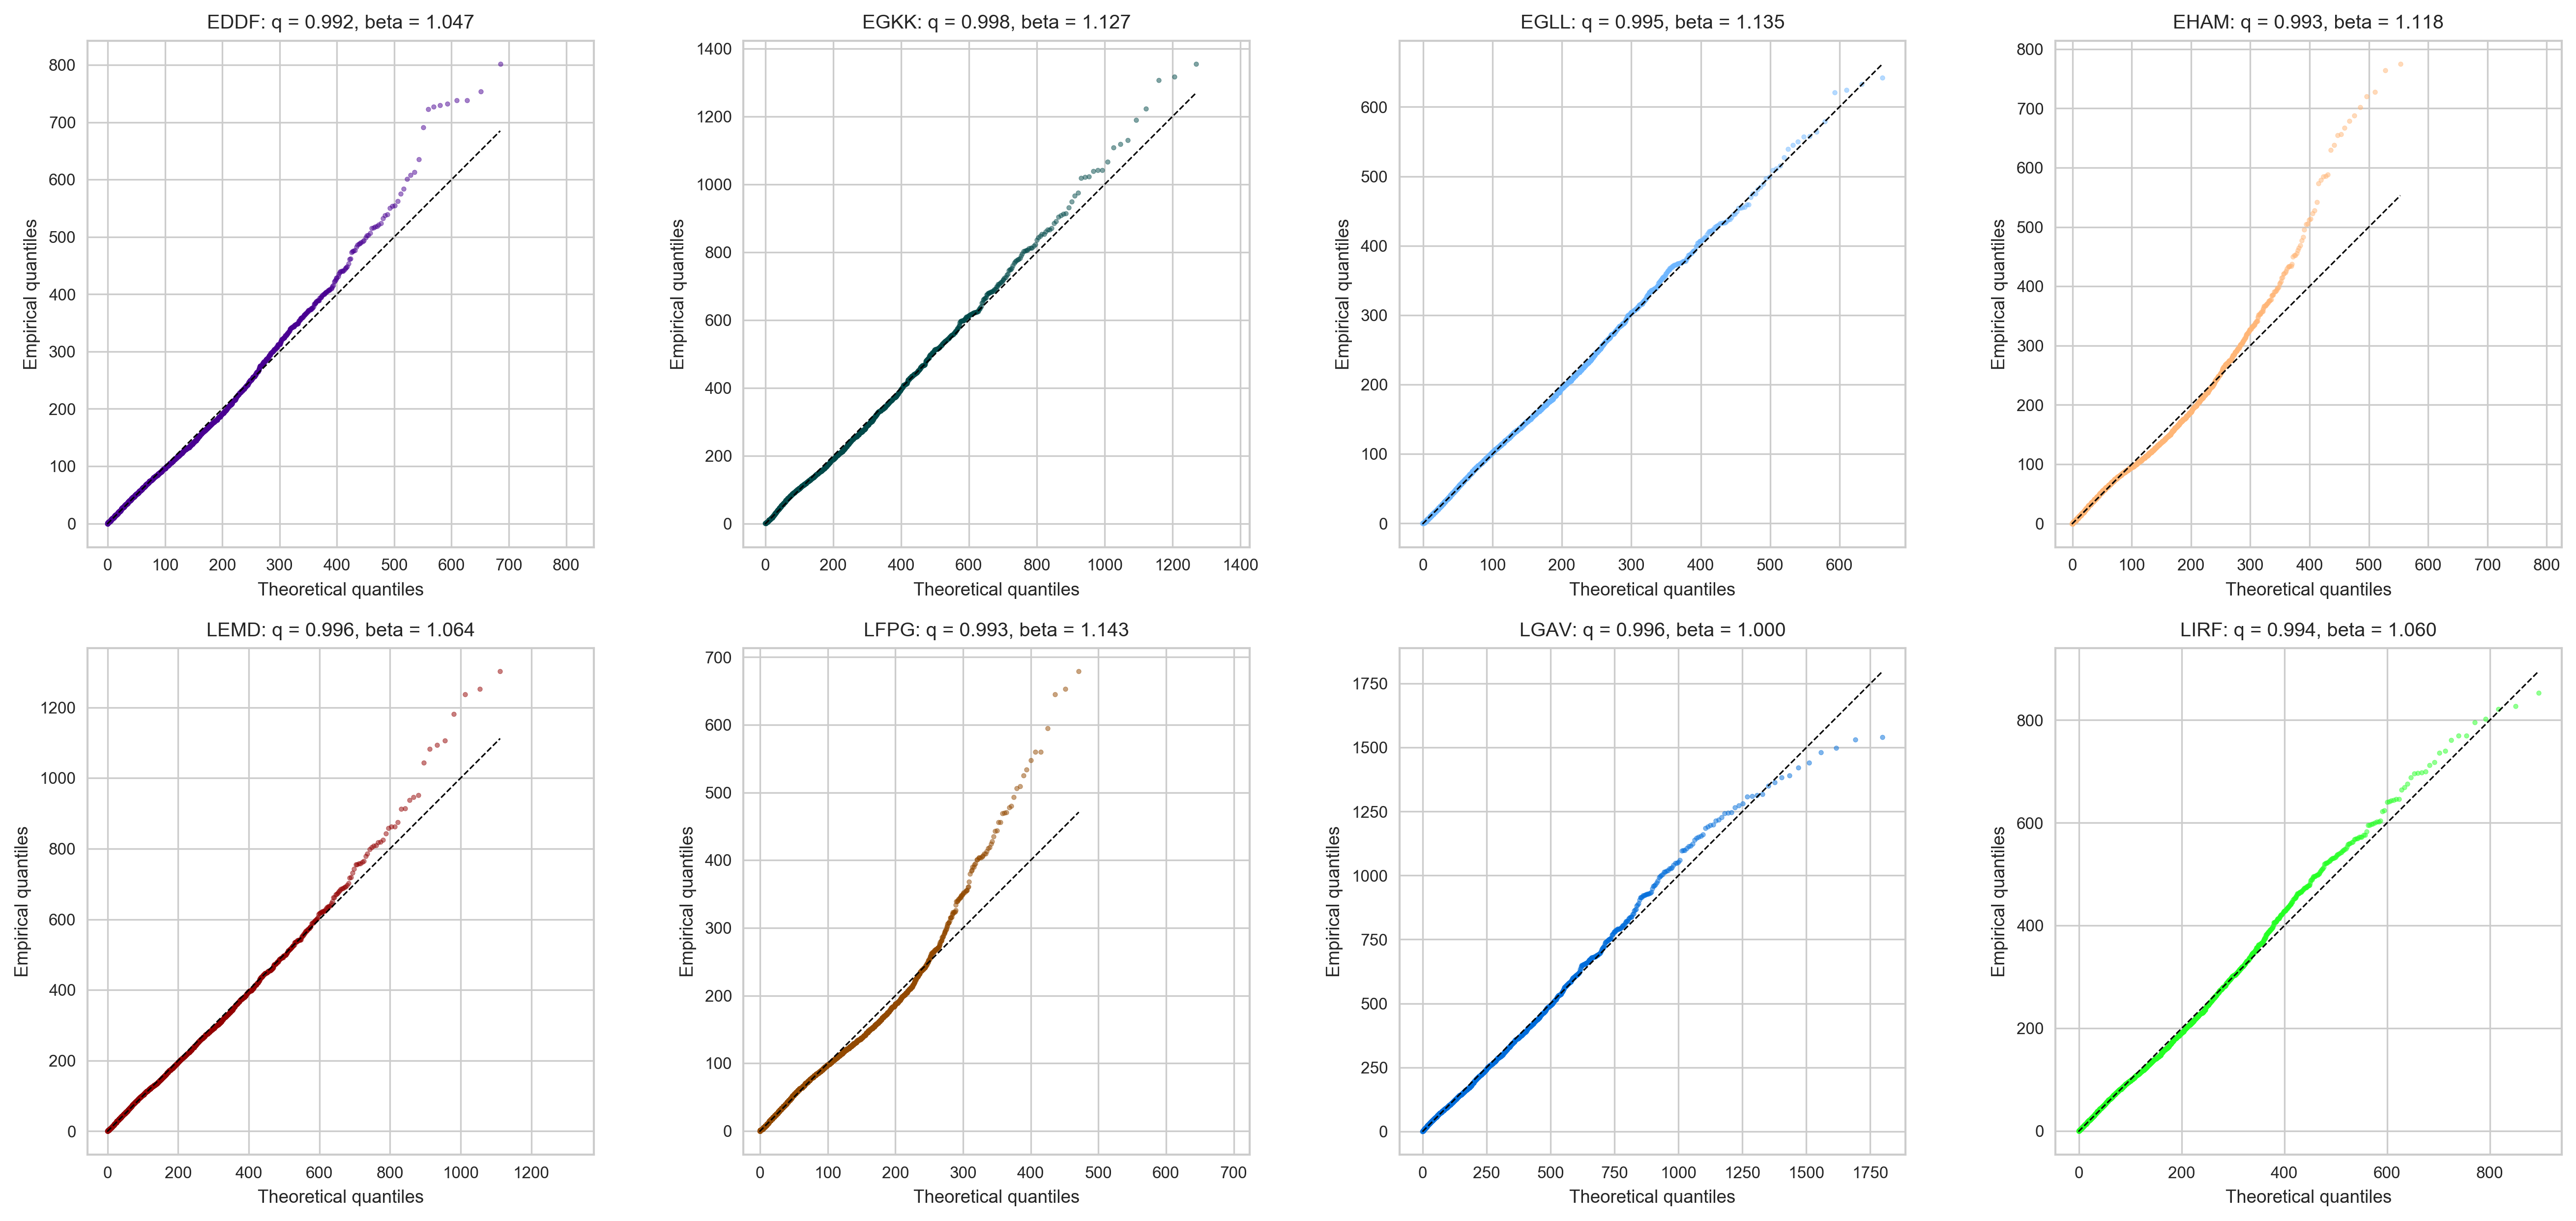
\includegraphics[width=\textwidth]{IA_qqplot0800-0930}
    \caption{QQ-plot of inter-arrivals at 40 NM in the period 08:00 -- 09:30. Theoretical quantiles obtained from~\eqref{eq:DWeibullPMF}; parameters listed in Table~\ref{tab:fitted}; times are local.}
    \label{fig:qqplot5-8}
\end{sidewaysfigure}

\begin{sidewaysfigure}
    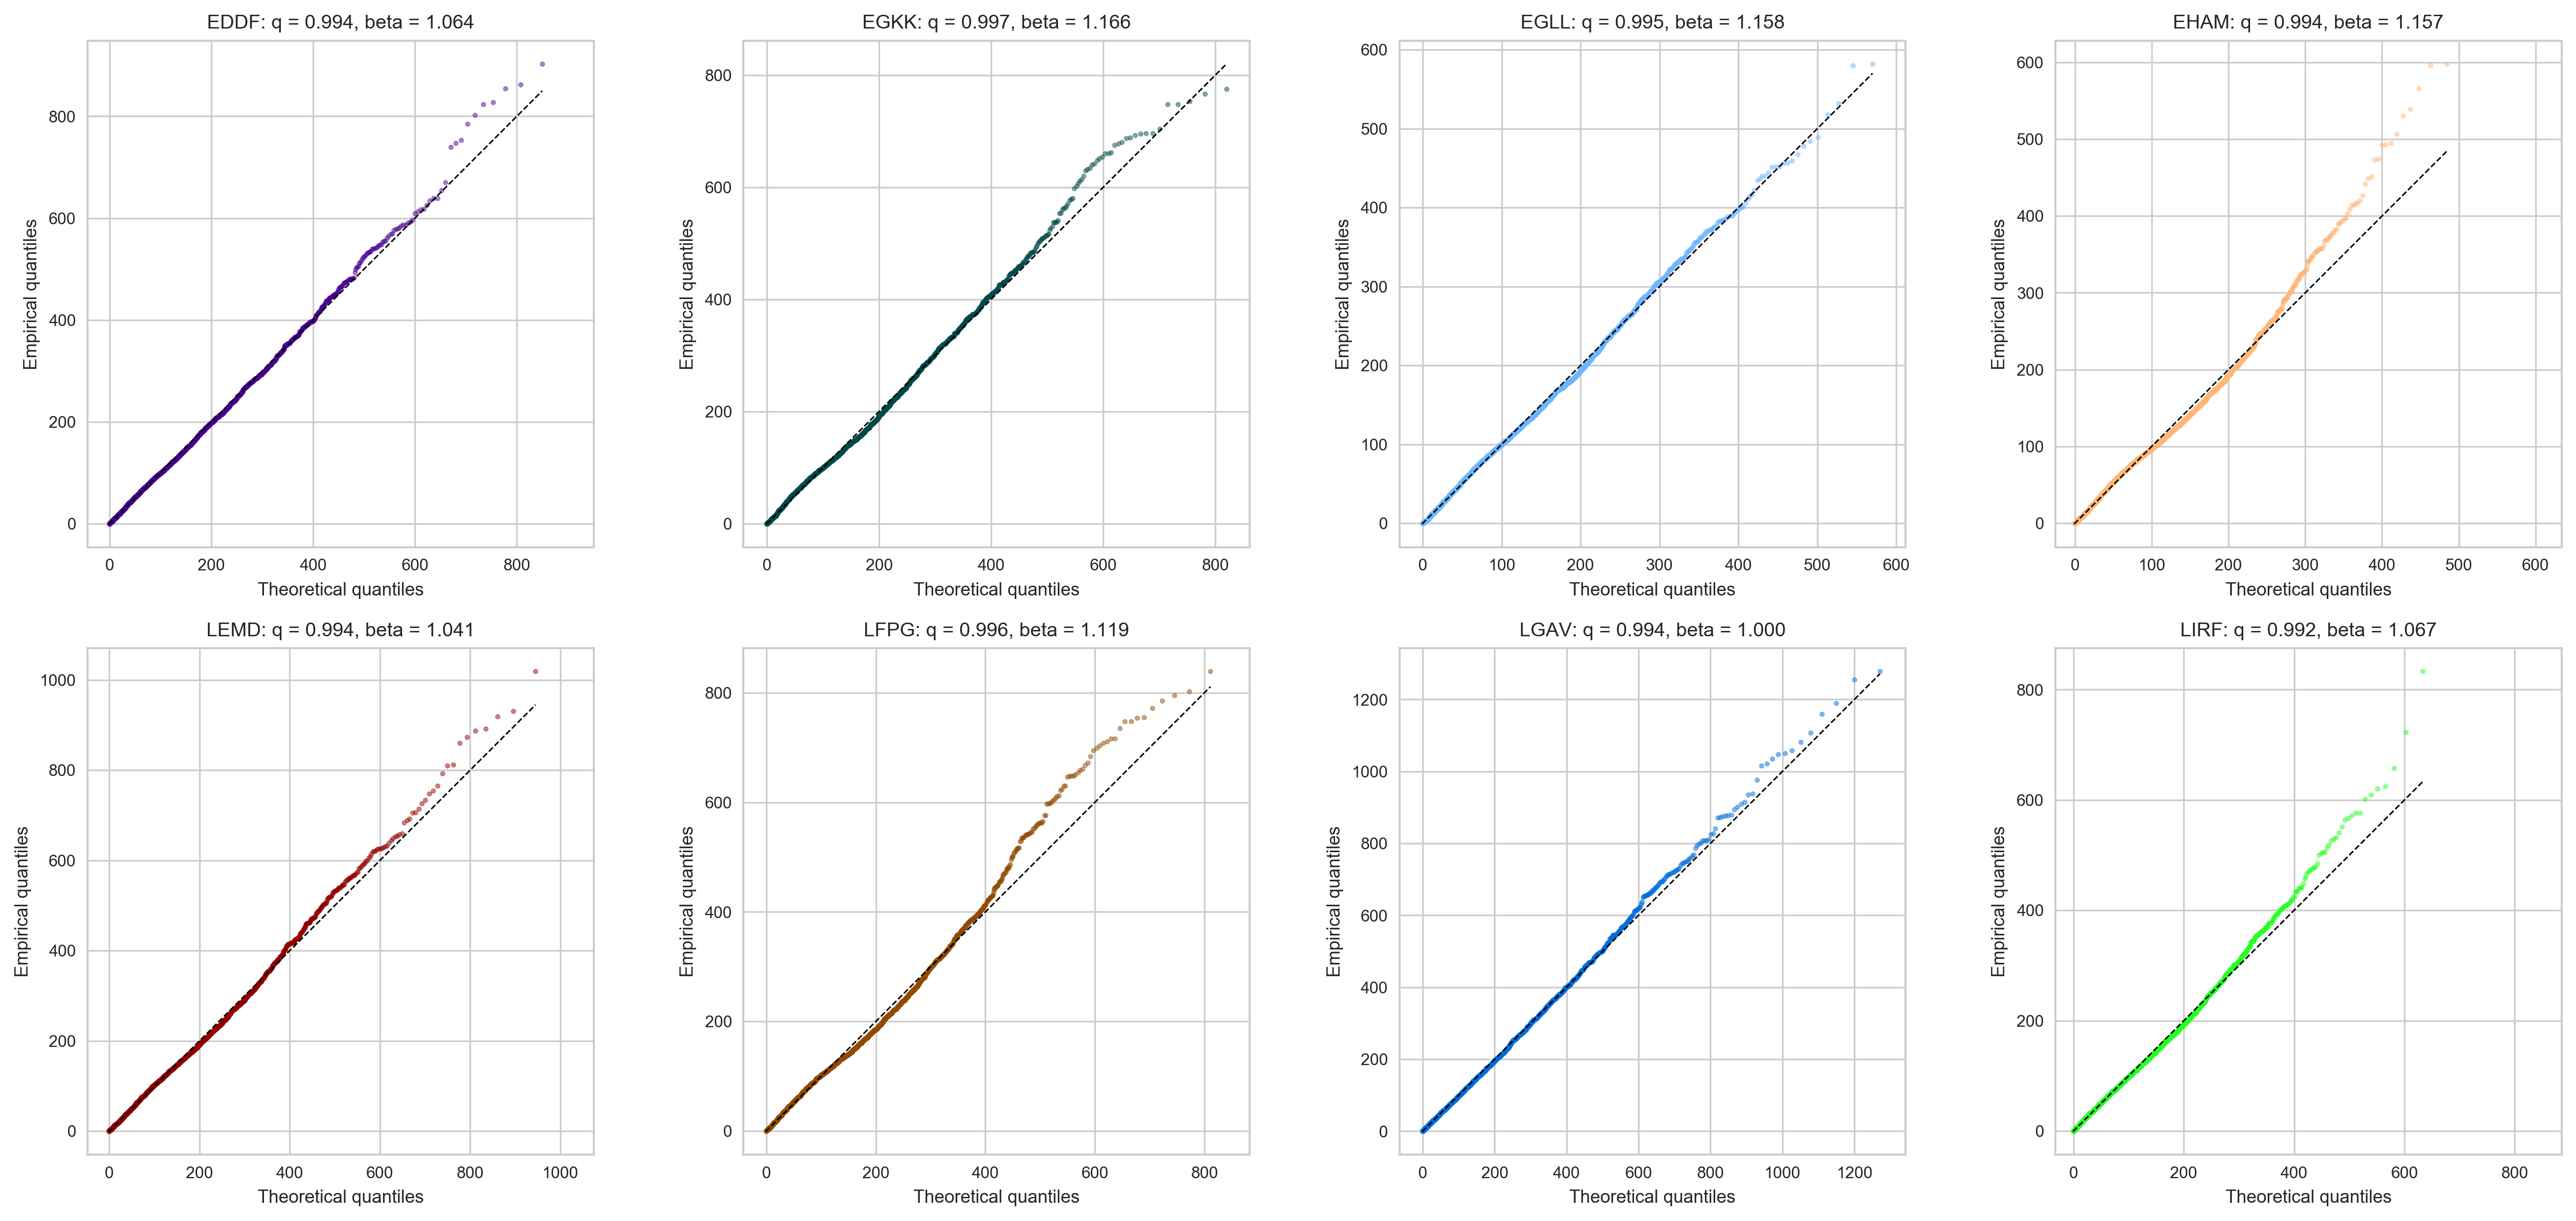
\includegraphics[width=\textwidth]{IA_qqplot1200-1330}
    \caption{QQ-plot of inter-arrivals at 40 NM in the period 12:00 -- 13:30 local time. Theoretical quantiles obtained from~\eqref{eq:DWeibullPMF}; parameters listed in Table~\ref{tab:fitted}; times are local.}
    \label{fig:qqplot5-11}
\end{sidewaysfigure}

\begin{sidewaysfigure}
    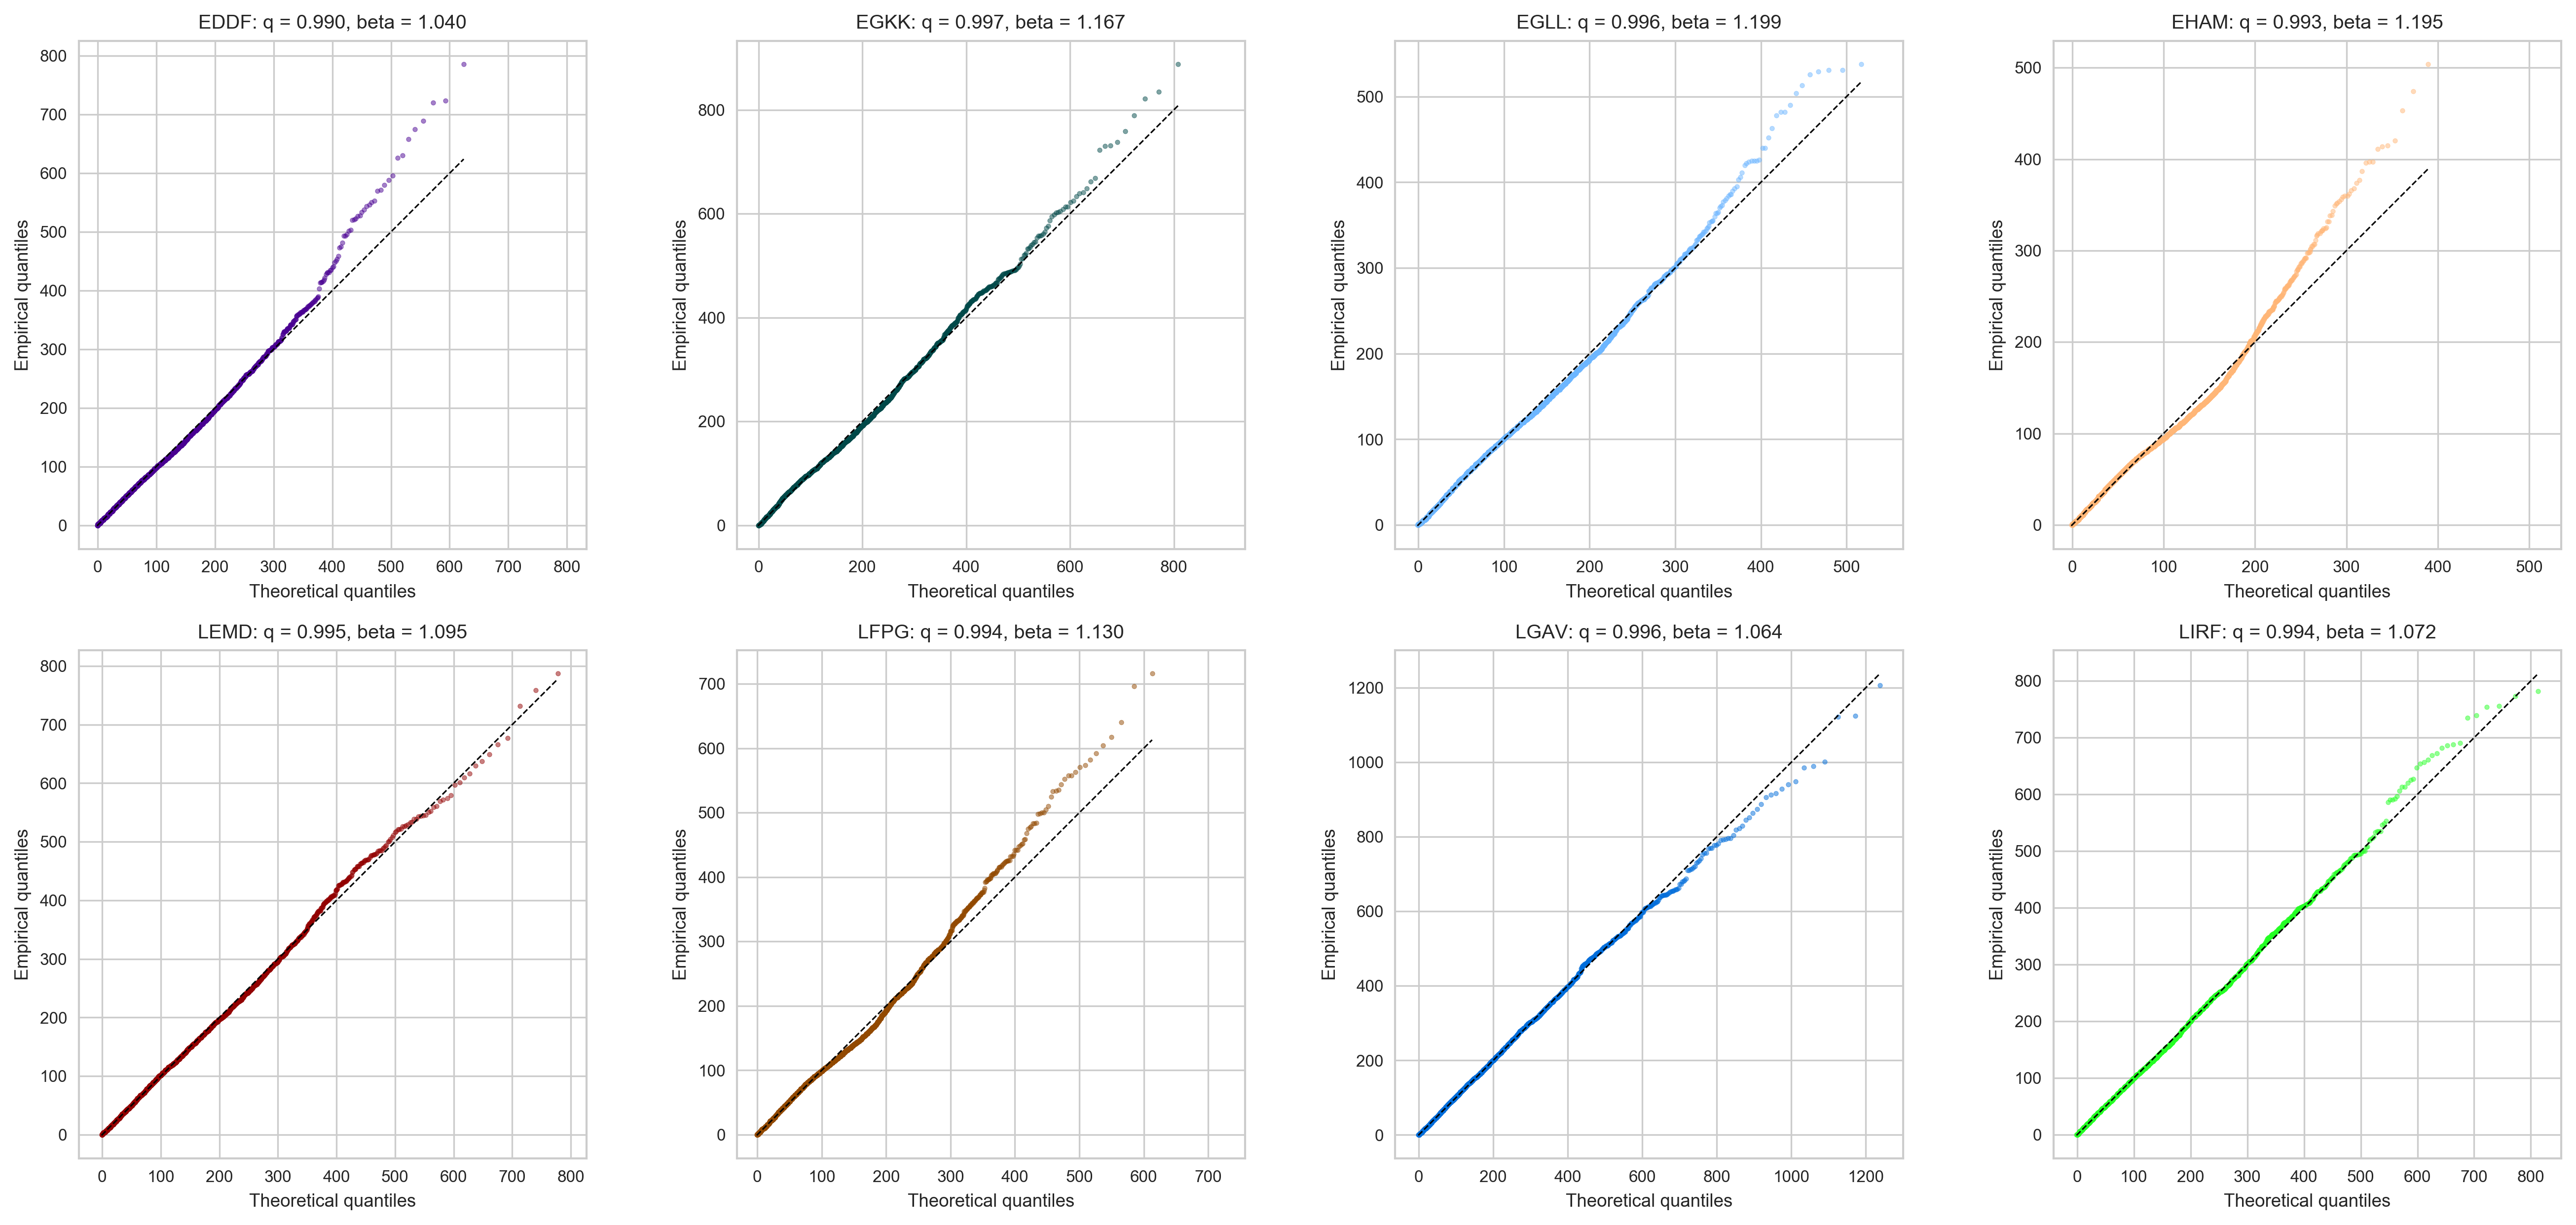
\includegraphics[width=\textwidth]{IA_qqplot1800-1930}
    \caption{QQ-plot of inter-arrivals at 40 NM in the period 18:00 -- 19:30 local time. Theoretical quantiles obtained from~\eqref{eq:DWeibullPMF}; parameters listed in Table~\ref{tab:fitted}; times are local.}
    \label{fig:qqplot5-17}
\end{sidewaysfigure}

\subsection{Arrival process: average demand and serial correlations}
\label{sec:serial_corr}

Figure~\ref{fig:AvgArrivals} shows the daily mean profile of the demand along its 95\% point-wise confidence band.
Most of the airports analyzed in this paper show the characteristic \emph{wavy pattern} for arrivals, typical of airports hosting hub-an-spoke operations.
A notable exception is \airp{lhr}, which has a fairly constant mean arrival rate and a corresponding arrival process that is characterized by a single regime: the demand oscillates around 7 arrivals every 10 minutes --the declared arrival capacity is 45 aircraft/hour.
This also explains why Heathrow shows the best fit with a nearly-exponential distribution in Figures~\ref{fig:qqplot5-8}--\ref{fig:qqplot5-17}.

%Figure~\ref{fig:AvgArrivals} shows the average demand over the day when aggregated by intervals of 10 minutes. The figure shows the mean number of arrivals along with 99\% pointwise confindence intervals. For many of the airports considered, the plot of the average daily arrivals shows the characteristic \emph{wavy pattern} typical of airports hosting hub-an-spoke operations. A notable exception is Heathrow, which has a nearly constant arrival rate and thus shows the best fit with a nearly-exponential distribution in Figures~\ref{fig:qqplot5-8}--\ref{fig:qqplot5-17}.
\begin{sidewaysfigure}
  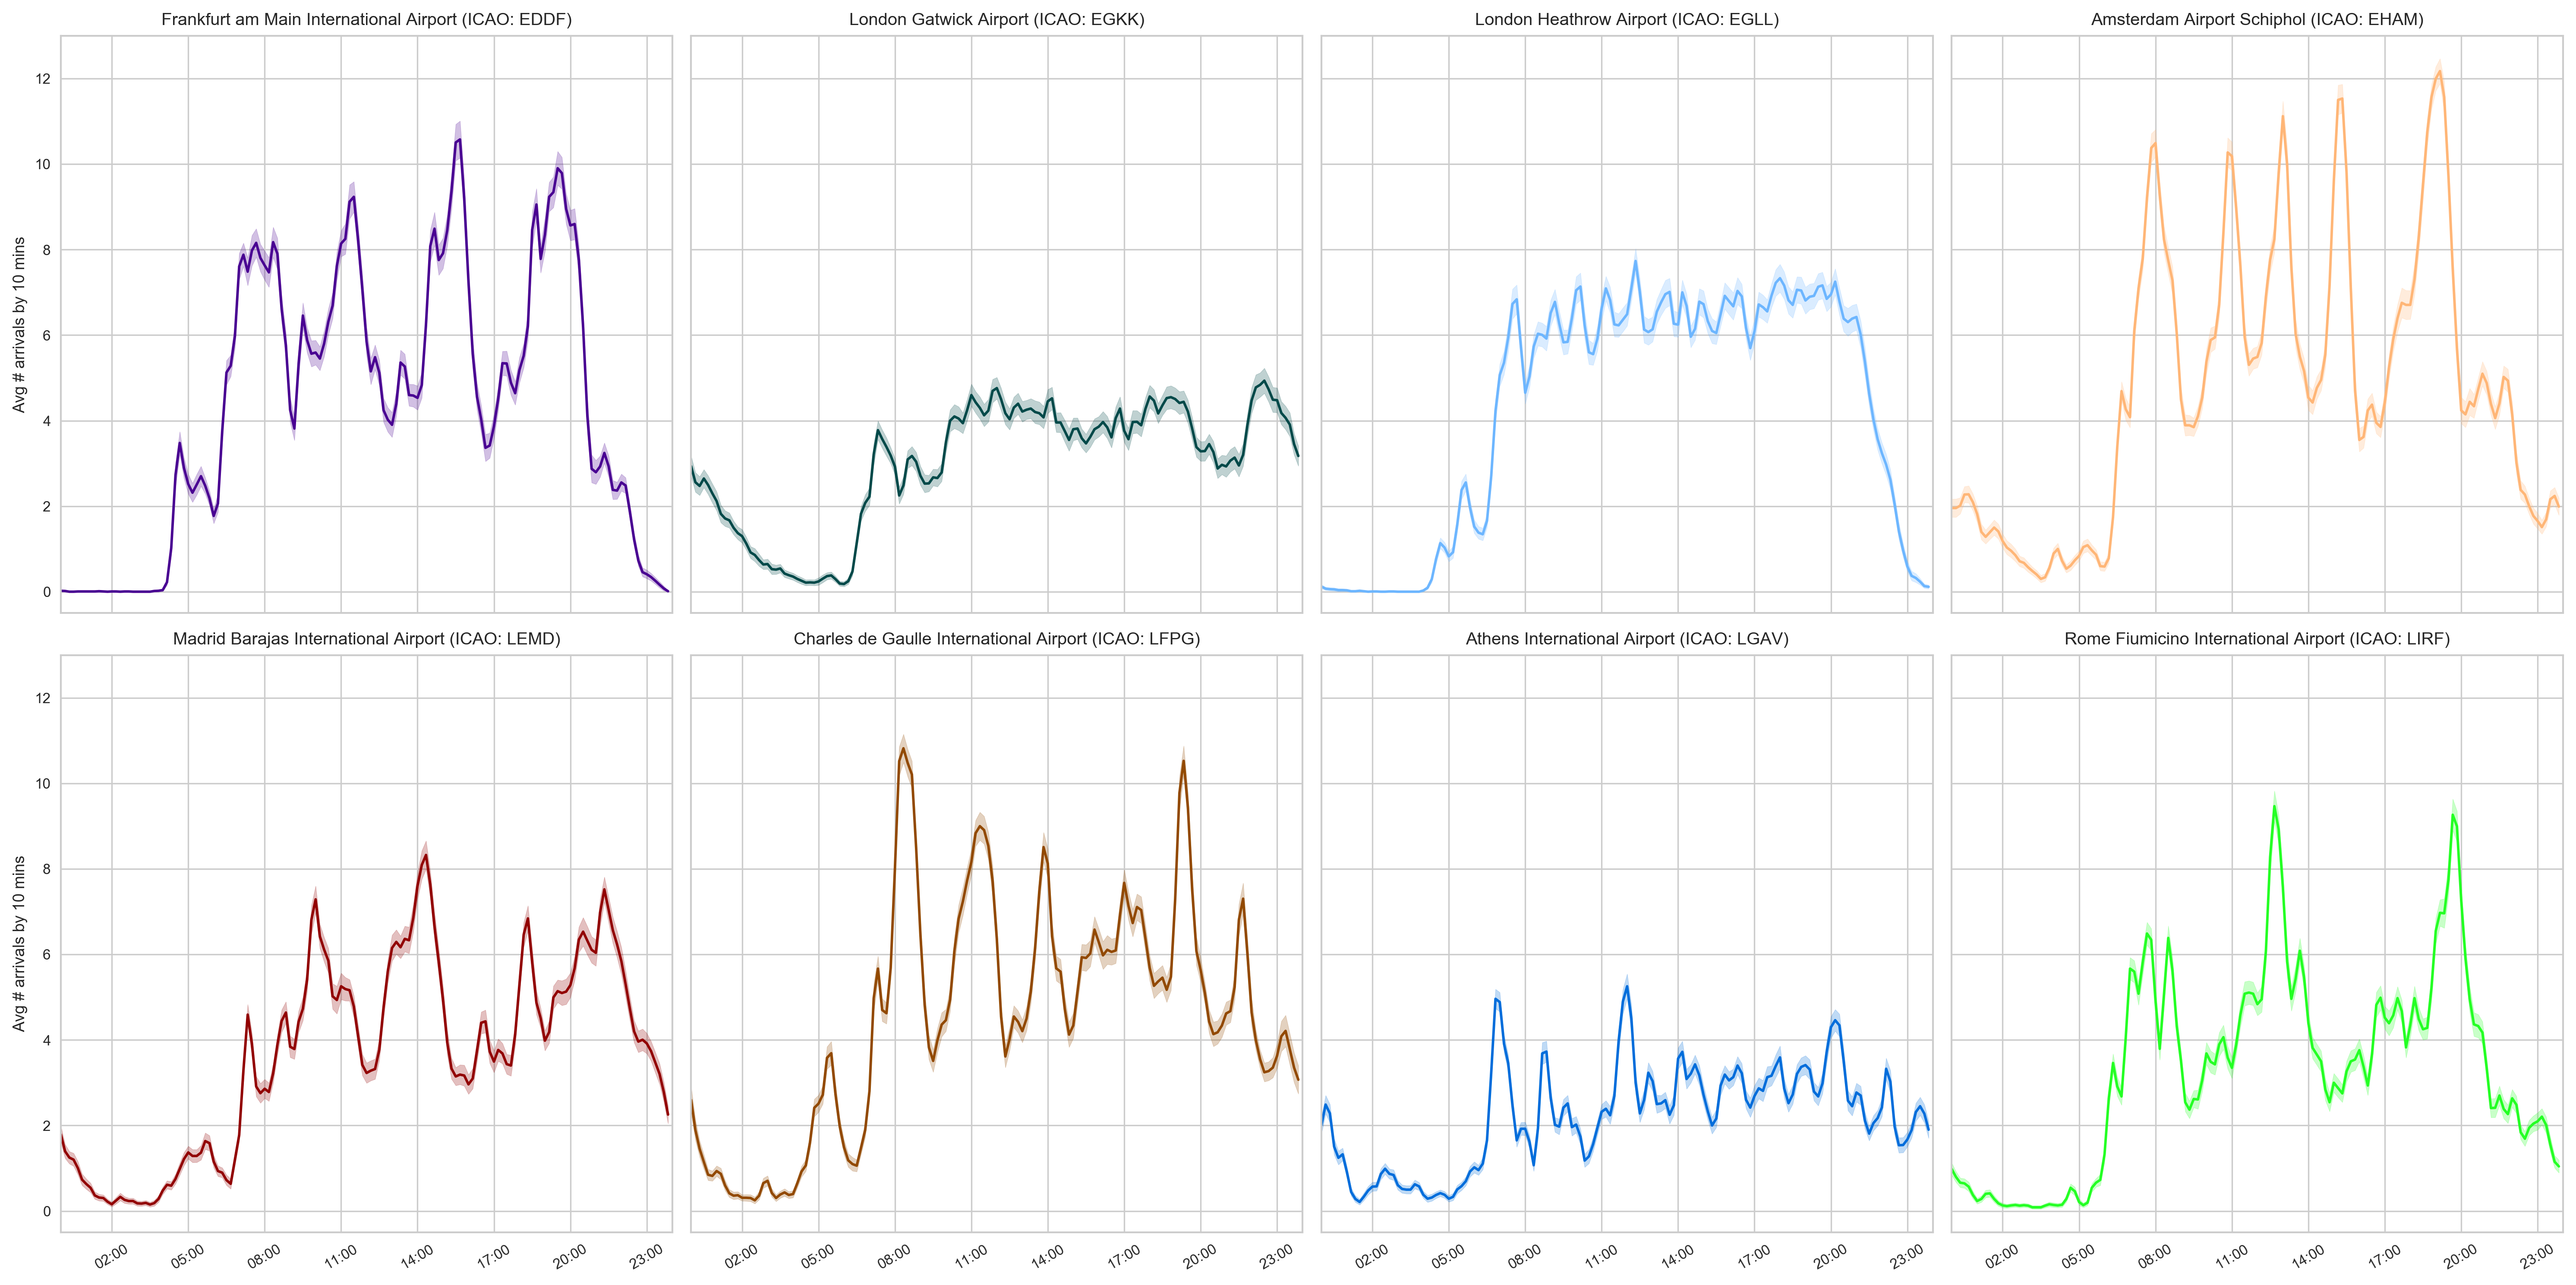
\includegraphics[width=\textwidth]{AvgArrivals}
  \caption{Average demand aggregated by 10 min. Shaded areas display 95\% point-wise confidence bands.}\label{fig:AvgArrivals}
\end{sidewaysfigure}

The correlograms in Figure~\ref{fig:autocorr} highlight the presence of two kinds of serial correlation in the demand.
First, all airports present a statistically significant strong negative lag-1 correlation.
These correlations cannot be appreciated in full from Figure~\ref{fig:autocorr} because the \(y\)-axis is clipped at \(\pm 0.2\) for making other correlations more readable. For this reason, their exact numerical value is reported in Table~\ref{tab:lag01}.
The presence of these correlations suggests that the net variation of the demand\footnote{The demand \ac{TS} is made stationary by taking first-order differences, see Section~\ref{sec:dm_serial_corr}.} over an interval of 10 minutes is negatively correlated with the demand variation in the following 10 minutes.
In other words, intervals where the demand increases (resp.\ decreases) are more likely to be followed by intervals where the demand decreases (resp.\ increases).
This property, which can also be guessed from Figure~\ref{fig:AvgArrivals}, might have an interesting connection with capacity constraints.
%and demonstrates that the demand is bounded by capacity.
In fact, if an interval of increased demand were likely followed by another interval of increased demand, then the capacity of the airport could be temporarily exceeded.

Second, many airports show the presence of statistically significant correlations at lags of 1, 2, and 3 days.
These correlations are not strong in absolute terms, yet they are the strongest shown by the correlograms, and their relatively low magnitude can be explained by the presence of natural daily variation of the demand evolution in a very large sample.
\ref{A-sec:appc} in the supplementary material offers a more-in-depth analysis of these serial correlations through a continuous wavelet transform of the demand. This analysis shows that correlations at lag of one or more days are of practical significance. Thus, we have the following:
\begin{kpt}\label{rmk:correlations}
  Significant correlations at lags multiple of one day motivate the idea of learning a daily-periodic non-homogeneous Poisson process in the next section.
\end{kpt}

\begin{sidewaysfigure}
  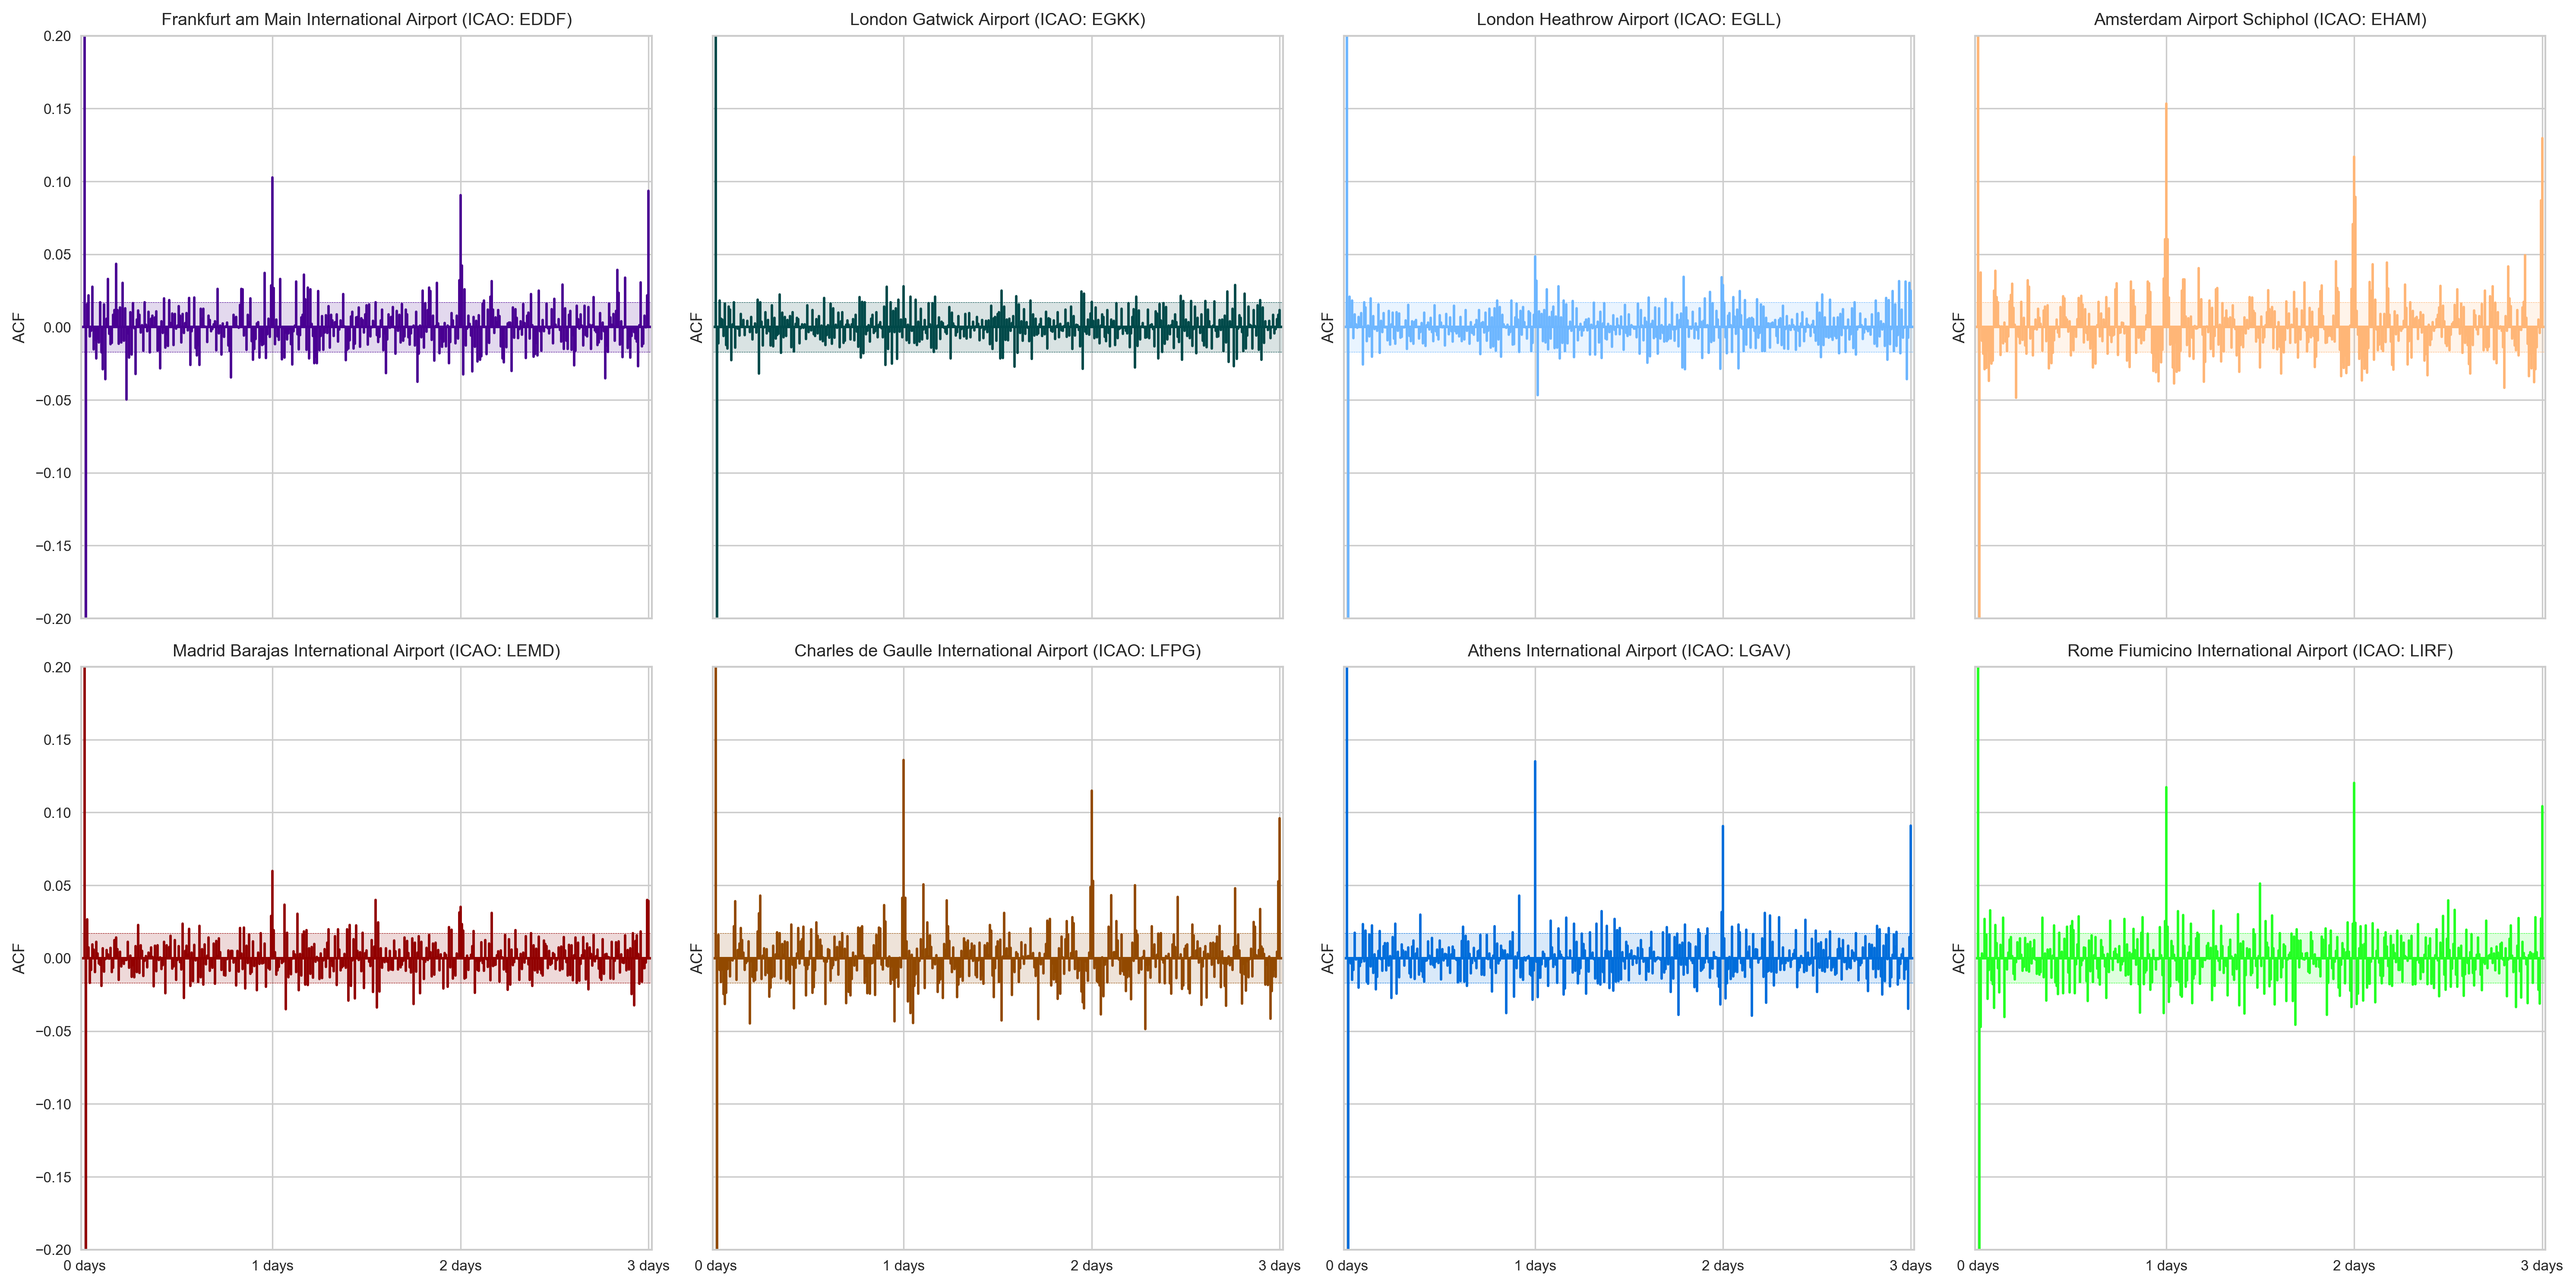
\includegraphics[width=\textwidth]{Autocorr}
  \caption{Autocorrelation of arrivals \ac{TS} aggregated by intervals of 10 minutes. Shared areas mark the limits of statistical significance at the 99\% level by Bartlett's Formula. For the sake of readability, the \(y\)-axis of the autocorrelation (1st column) is capped at \(\pm 0.2\). The values of the lag-0 and lag-1 correlations are off scale, and the latter aereported by Table~\ref{tab:lag01}.}\label{fig:autocorr}
\end{sidewaysfigure}

\begin{table}[tbp]
  \centering
  \caption{Values of lag-1 autocorrelations.}\label{tab:lag01}
  \begin{tabular}{lr}
    \toprule
    \acs{IATA} code & lag-1 autocorr.\\
    \midrule
    \airp{fra} & -0.447\\
    \airp{lgw} & -0.526\\
    \airp{lhr} & -0.440\\
    \airp{ams} & -0.359\\
    \airp{mad} & -0.466\\
    \airp{cgd} & -0.415\\
    \airp{ath} & -0.479\\
    \airp{fco} & -0.535\\
    \bottomrule
  \end{tabular}
\end{table}

Figure~\ref{fig:correlations_true} shows the Pearson's correlation \(\rho_{t_i, t_{i+1}}\) between the \emph{demand variation} in the intervals \([t_i, t_{i+1})\) and \([t_{i+1}, t_{i+2})\).
The demand variation is computed as the difference between the number of arrivals observed from \(t^{a}_i\) data and the number of arrivals that were expected according to \(t^{r}_i\) data.
The value of \(\rho_{t_i, t_{i+1}}\) is mostly negative, especially during normal operations hours.
The majority of these correlations are different or borderline-different from zero at a 5\% significance level.
This finding is expected in view of the lag-1 autocorrelations reported by Table~\ref{tab:lag01}.
\begin{kpt}
	The sign of the correlations is in line with the general result that \ac{PSRA} generate negatively autocorrelated streams~\citep{guadagni2011queueing}.
  Please note that~\citet{guadagni2011queueing} compute correlations from the observed inbound stream, but have a equally-spaced-in-time arrival schedule.  In our formulation, pre-scheduled arrivals are not equally spaced, but come from the regulated flight plan.
  Accordingly, the correct quantity to consider is the demand variation.
\end{kpt}
% \begin{rmk}
%   Please note that~\citet{guadagni2011queueing} compute correlations from the observed inbound stream, but have a equally-spaced-in-time arrival schedule.  In our formulation, pre-scheduled arrivals are not equally spaced, but come from the M1 flight plan.
%   Accordingly, the correct quantity to consider is the demand variation.
% \end{rmk}

% On this key point, it is important to observe  that~\citet{guadagni2011queueing} compute correlations from the observed inbound stream, but have a equally-spaced-in-time arrival schedule.

% \begin{kpt}
  The negative sign of correlations is a very appealing feature of the model as it reflects bounds on the available capacity of both terminal airspace and arrival airport.
  If demand variations were mostly uncorrelated or even positively correlated, random fluctuations in the inbound flow might temporarily exceed the capacity of airports and/or terminal sectors.
  On the contrary, the regulated schedule imposes a structure in the sequence of arrivals~\eqref{eq:psra-like}.
% \end{kpt}
For the sake of completeness, correlations computed on simulations of~\ref{eq:psra-like} are shown in~\ref{A-sec:appb} of the supplementary material.

\begin{sidewaysfigure}
    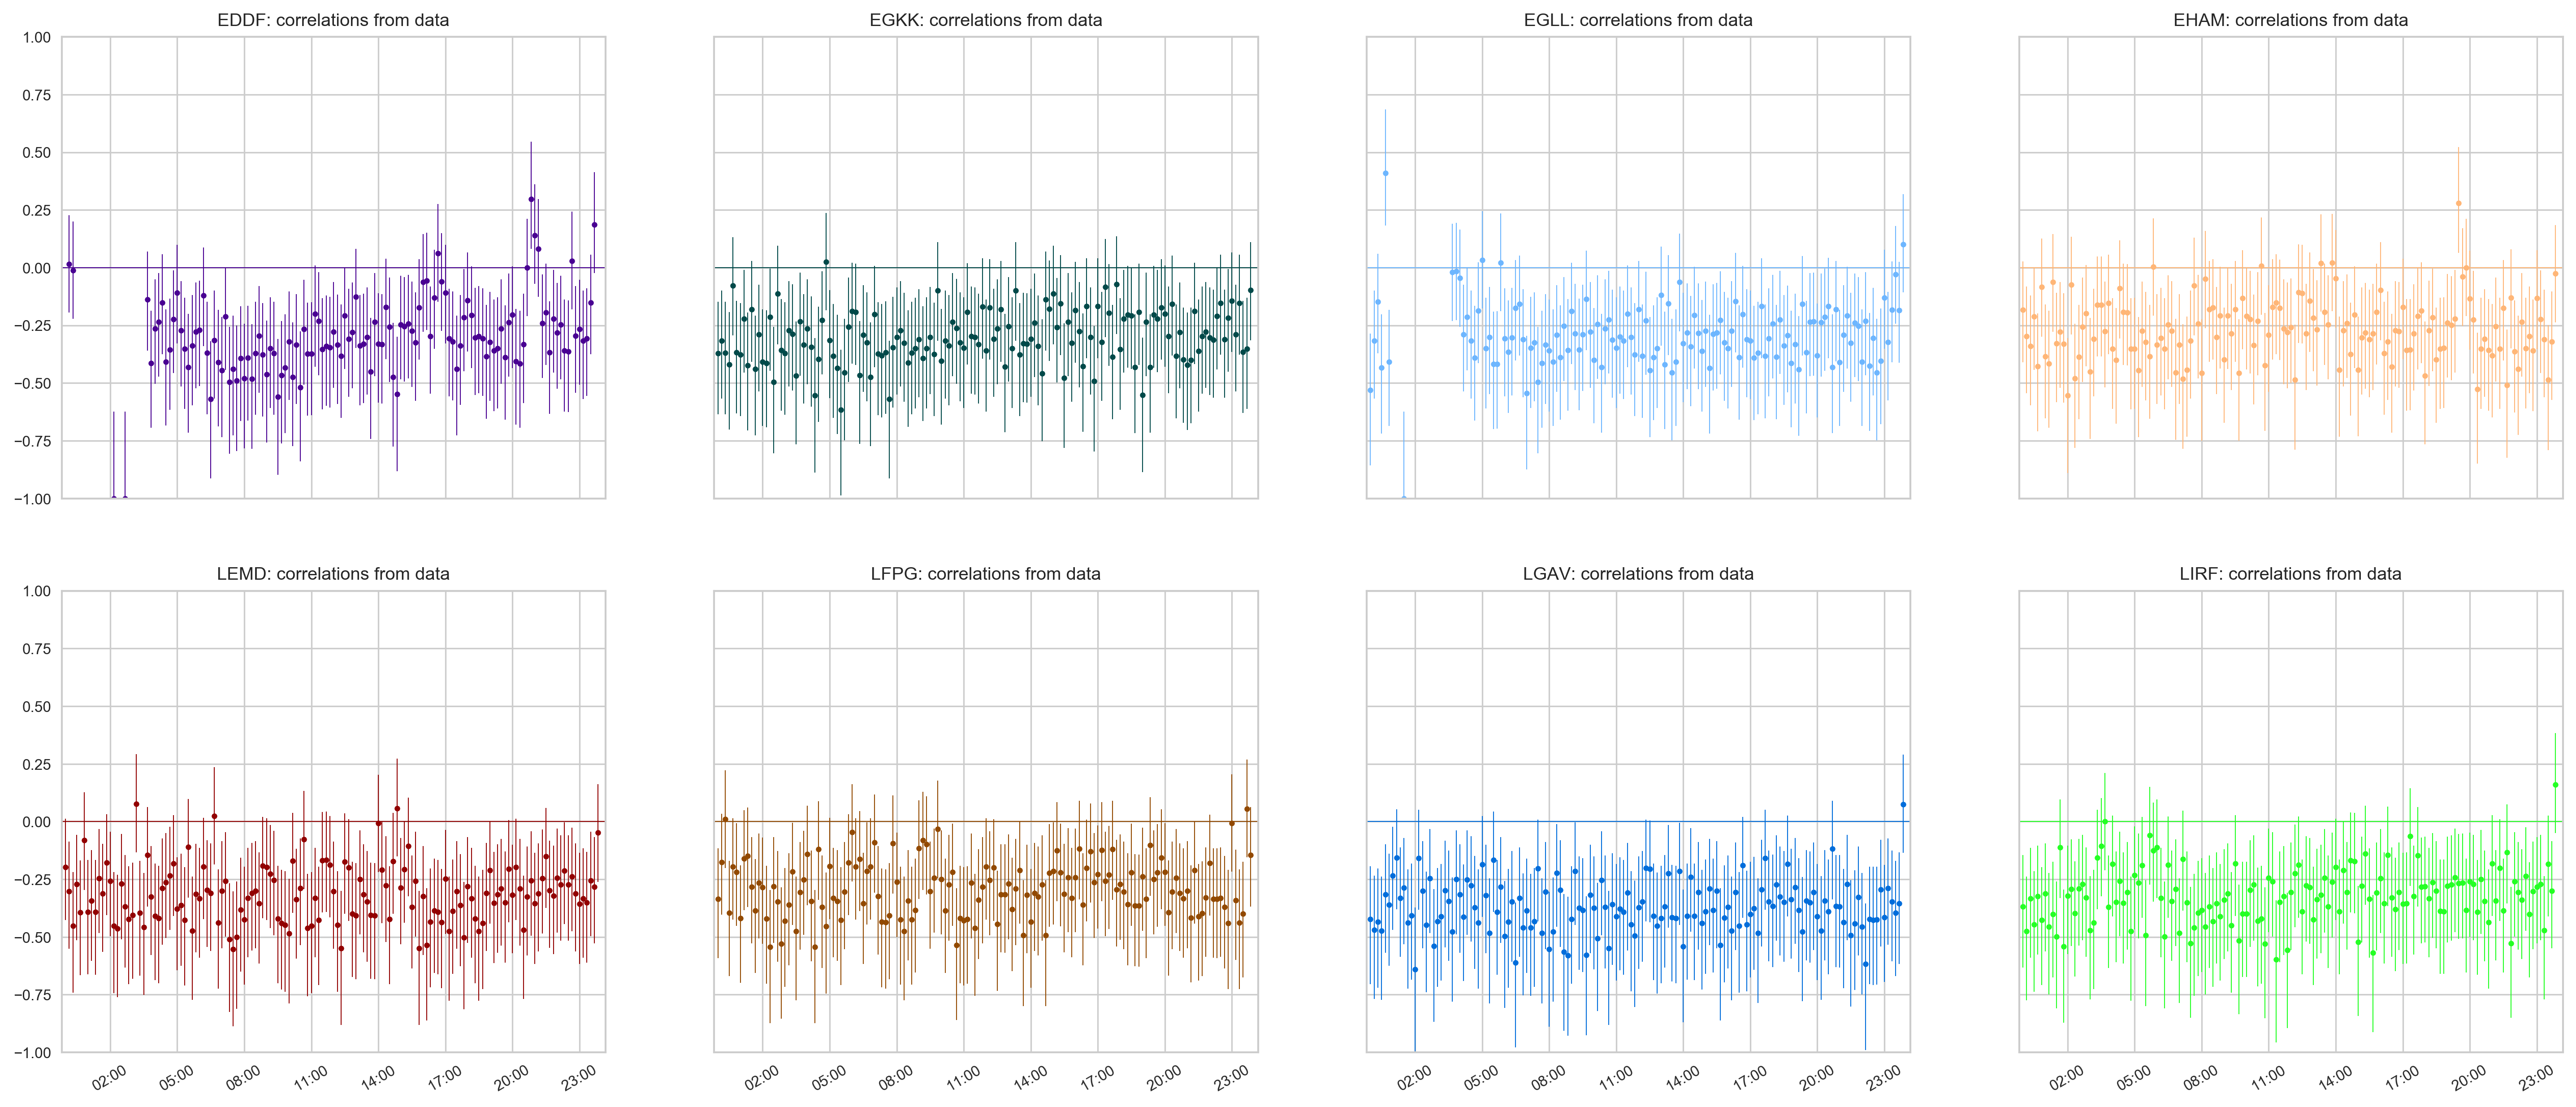
\includegraphics[width=\textwidth]{correlations_true}
    \caption{Correlations from \(t^{a}_i\) data. Error bars show 95\% confidence interval for Pearson's \(\rho\).}
    \label{fig:correlations_true}
\end{sidewaysfigure}

\subsection{Data-driven modeling of the arrival processes}\label{sec:modeling}

Using the data-driven methodology described in Section~\ref{sec:dm_modeling}, we now detail the parameters characterizing the inbound-stream models, \ie{} non-homogeneous Poisson and \ac{PSRA}, at the considered airport.
We begin with the construction of the Poisson process, which is daily-periodic in our formulation.
This modeling choice is motivated by Key Point~\ref{rmk:correlations} above.

\subsubsection{Construction of the non-homogeneous Poisson process}\label{sec:pois}

Figure~\ref{fig:poisson_segmentation} shows the \DBSCAN{} clustering of change-points identified by \PELT{} and the daily average rate of arrivals at 40 NM per 10-minute  intervals.
For each cluster, thin dashed lines mark the average time of the day \(\hat{t}_i\) and the corresponding average Poisson intensity \(\hat{\lambda}_i\), where \(i\) is the index of the cluster.
In view of the 24-hour periodicity of the demand highlighted in Section~\ref{sec:serial_corr}, we define our data-driven in-homogeneous Poisson model by a periodic step-function, which takes on value \(\hat{\lambda}_i\) for \(\hat{t}_i \leq t < \hat{t}_{i+1}\).
The values of \(\hat{t}_i\) and \(\hat{\lambda}_i\) are reported by Table~\ref{A-tab:poisson_segmentation} in~\ref{A-sec:appd} of the supplementary material.

\begin{rmk}
	Note that the values of \(\hat{\lambda}\) are substantially in line with the fitted values from Table~\ref{tab:fitted}, since \(\lambda \approx 60 \times \text{mean}^{-1}\) in the approximation of exponential inter-arrivals.
\end{rmk}
%%%%%%%%%%%%%%%

\begin{sidewaysfigure}
    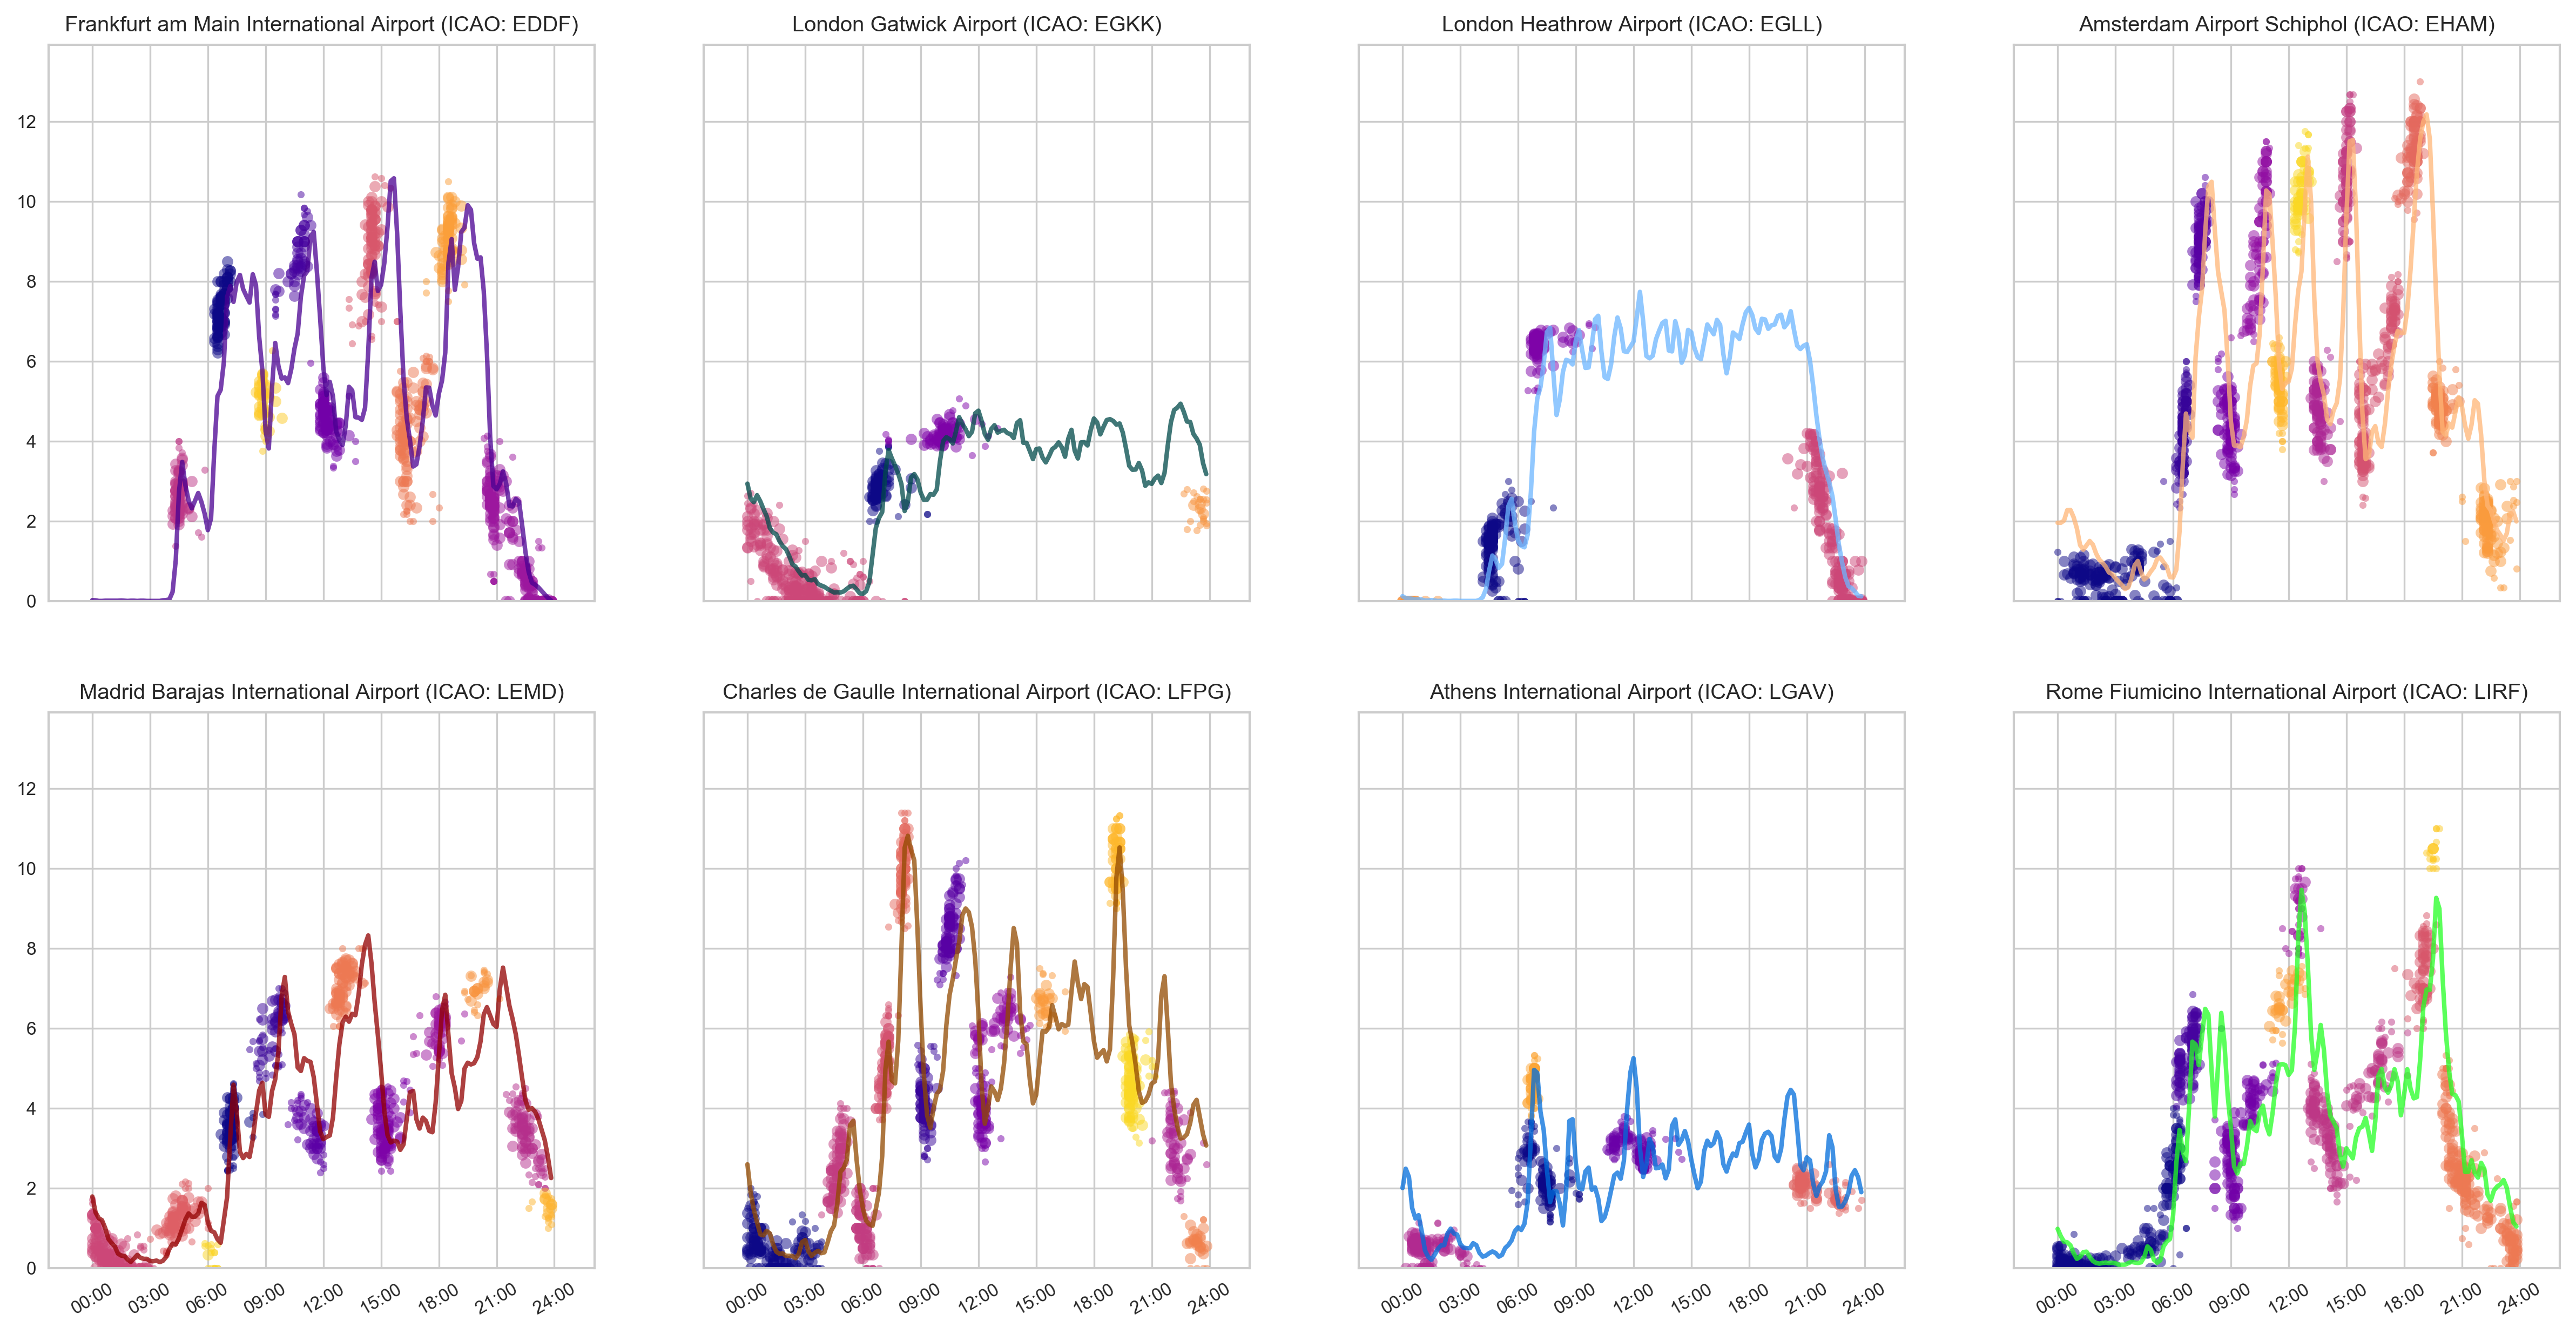
\includegraphics[width=\textwidth]{DDPoisson}
    \caption{Result of \DBSCAN{} clustering after \PELT{} changepoint analysis. Points belonging to the same clusters are coloured with the same colour. The clustering result is shown superimposed to the daily average from Figure~\ref{fig:AvgArrivals}.}\label{fig:poisson_segmentation}
\end{sidewaysfigure}

\subsubsection{Construction of the \acs{PSRA} process}\label{sec:psra}

Tables~\ref{tab:inner_cv} and~\ref{tab:outer_cv} show the results of a nested cross validation of \ac{PSRA} process~\eqref{eq:psra-like}, where the delays \(\xi_i\) are obtained via a regression model.
The model is validated on its capability of predicting the aggregated demand and not the delays \(\xi_i\).
Based on 5 consecutive two-weekly splits, the inner cross validation estimates the best parameters \(C\) and \(\varepsilon\) of the support vector machine on a logarithmic grid \(C = 10^{-2},\ldots, 10^5; \varepsilon = 10^{-5},\dots,10^2\).
The outer cross validation evaluates demand prediction on a 11-fold cross validation based on consecutive weekly splits.
The \(r^2\) metric is often around 0.5, meaning that the model is capturing a good part of the variance of the demand, while the mean absolute error is about 1.5 aircraft/10 minutes.
\begin{kpt}
  It is clear that even a simple regression model like the one used for the delays is performing quite well.
\end{kpt}

\begin{table}
  \caption{Inner cross-validation of \acs{PSRA} model~\eqref{eq:psra-like}. The table shows the best values for the parameters of the support vector machine regression model using a sequential two-weekly split, and the corresponding average values of \acl{MAE} (\acs{MAE}), \acl{MSE} (\acs{MSE}), and \(r^2\) using 11-fold consecutive weekly splits.}\label{tab:inner_cv}
  \centering
  \begin{tabular}{lrrrrr}
    \toprule
    airport &       C &    \(\varepsilon\) &       \acs{MAE} &       \acs{MSE} &        \(r^2\) \\
    \midrule
    \airp{fra} &   100.0 &  100.000 &  0.055680 &  0.330237 &  0.034639 \\
    \airp{lgw} &  1000.0 &    0.001 &  0.024724 &  0.088728 &  0.027090 \\
    \airp{lhr} &   100.0 &    0.100 &  0.042192 &  0.257391 &  0.026009 \\
    \airp{ams} &    10.0 &  100.000 &  0.037729 &  0.296439 &  0.023622 \\
    \airp{mad} &   100.0 &  100.000 &  0.042015 &  0.205384 &  0.024280 \\
    \airp{cgd} &   100.0 &    0.010 &  0.025096 &  0.147226 &  0.018576 \\
    \airp{ath} &  1000.0 &    1.000 &  0.034228 &  0.119433 &  0.042989 \\
    \airp{fco} &  1000.0 &    1.000 &  0.024727 &  0.146581 &  0.026880 \\
    \bottomrule
  \end{tabular}
\end{table}

\begin{table}
  \caption{Outer cross-validation of \acs{PSRA} model~\eqref{eq:psra-like}. The table shows average value (\(\mu\)) and standard deviation (\(\sigma\)) of \acl{MAE} (\acs{MAE}), \acl{MSE} (\acs{MSE}), and \(r^2\) using 11-fold consecutive weekly splits.}
  \label{tab:outer_cv}
  \centering
  \begin{tabular}{lrrrrrr}
    \toprule
    airport &  \acs{MAE} (\(\mu\)) &  \acs{MAE} (\(\sigma\)) &  \acs{MSE} (\(\mu\)) &  \acs{MSE} (\(\sigma\)) &  \(r^2\) (\(\mu\)) &  \(r^2\) (\(\sigma\)) \\
    \midrule
    \airp{fra} & 1.591 & 0.071 & 5.531 & 0.366 & 0.594 & 0.036 \\
    \airp{lgw} & 1.436 & 0.043 & 3.911 & 0.204 & 0.126 & 0.069 \\
    \airp{lhr} & 1.582 & 0.061 & 5.414 & 0.370 & 0.509 & 0.033 \\
    \airp{ams} & 1.831 & 0.078 & 6.490 & 0.530 & 0.530 & 0.041 \\
    \airp{mad} & 1.563 & 0.044 & 4.765 & 0.281 & 0.378 & 0.035 \\
    \airp{cgd} & 1.700 & 0.059 & 5.477 & 0.323 & 0.500 & 0.033 \\
    \airp{ath} & 1.199 & 0.040 & 2.752 & 0.156 & 0.141 & 0.052 \\
    \airp{fco} & 1.356 & 0.037 & 3.844 & 0.143 & 0.514 & 0.026 \\
    \bottomrule
  \end{tabular}
\end{table}

\subsection{Prediction capabilities of data-driven Poisson and \acs{PSRA}}\label{sec:comparison}

The prediction capabilities of both in-homogeneous Poisson and \ac{PSRA} are compared by Figures~\ref{fig:pred_last_week} and~\ref{fig:pred_last_day}.
The first figure shows the average-demand prediction obtained for the last week included in the dataset (September 5--11, 2016), while the second figure shows the prediction of the demand for the last day (September 14, 2016).
Results are plotted as difference between true and predicted demand (solid: \ac{PSRA}, dotted: Poisson).
Figure~\ref{fig:pred_last_week} clearly shows that \ac{PSRA} are much more accurate than Poisson in predicting the average future demand.
Table~\ref{tab:predictions_last_day} compares models by presenting \ac{MAE}, \ac{MSE}, and \(r^2\) score for this prediction task at each airport.
A close look at Figure~\ref{fig:pred_last_day} shows that, for the prediction on a single day, the demand predicted by the Poisson model fluctuates more than \ac{PSRA} around the true value.
Table~\ref{tab:predictions_last_day} shows indeed that \ac{PSRA} still have a higher predictive accuracy also in this task, due to a smaller error and a higher \(r^2\) score.

\begin{sidewaysfigure}
    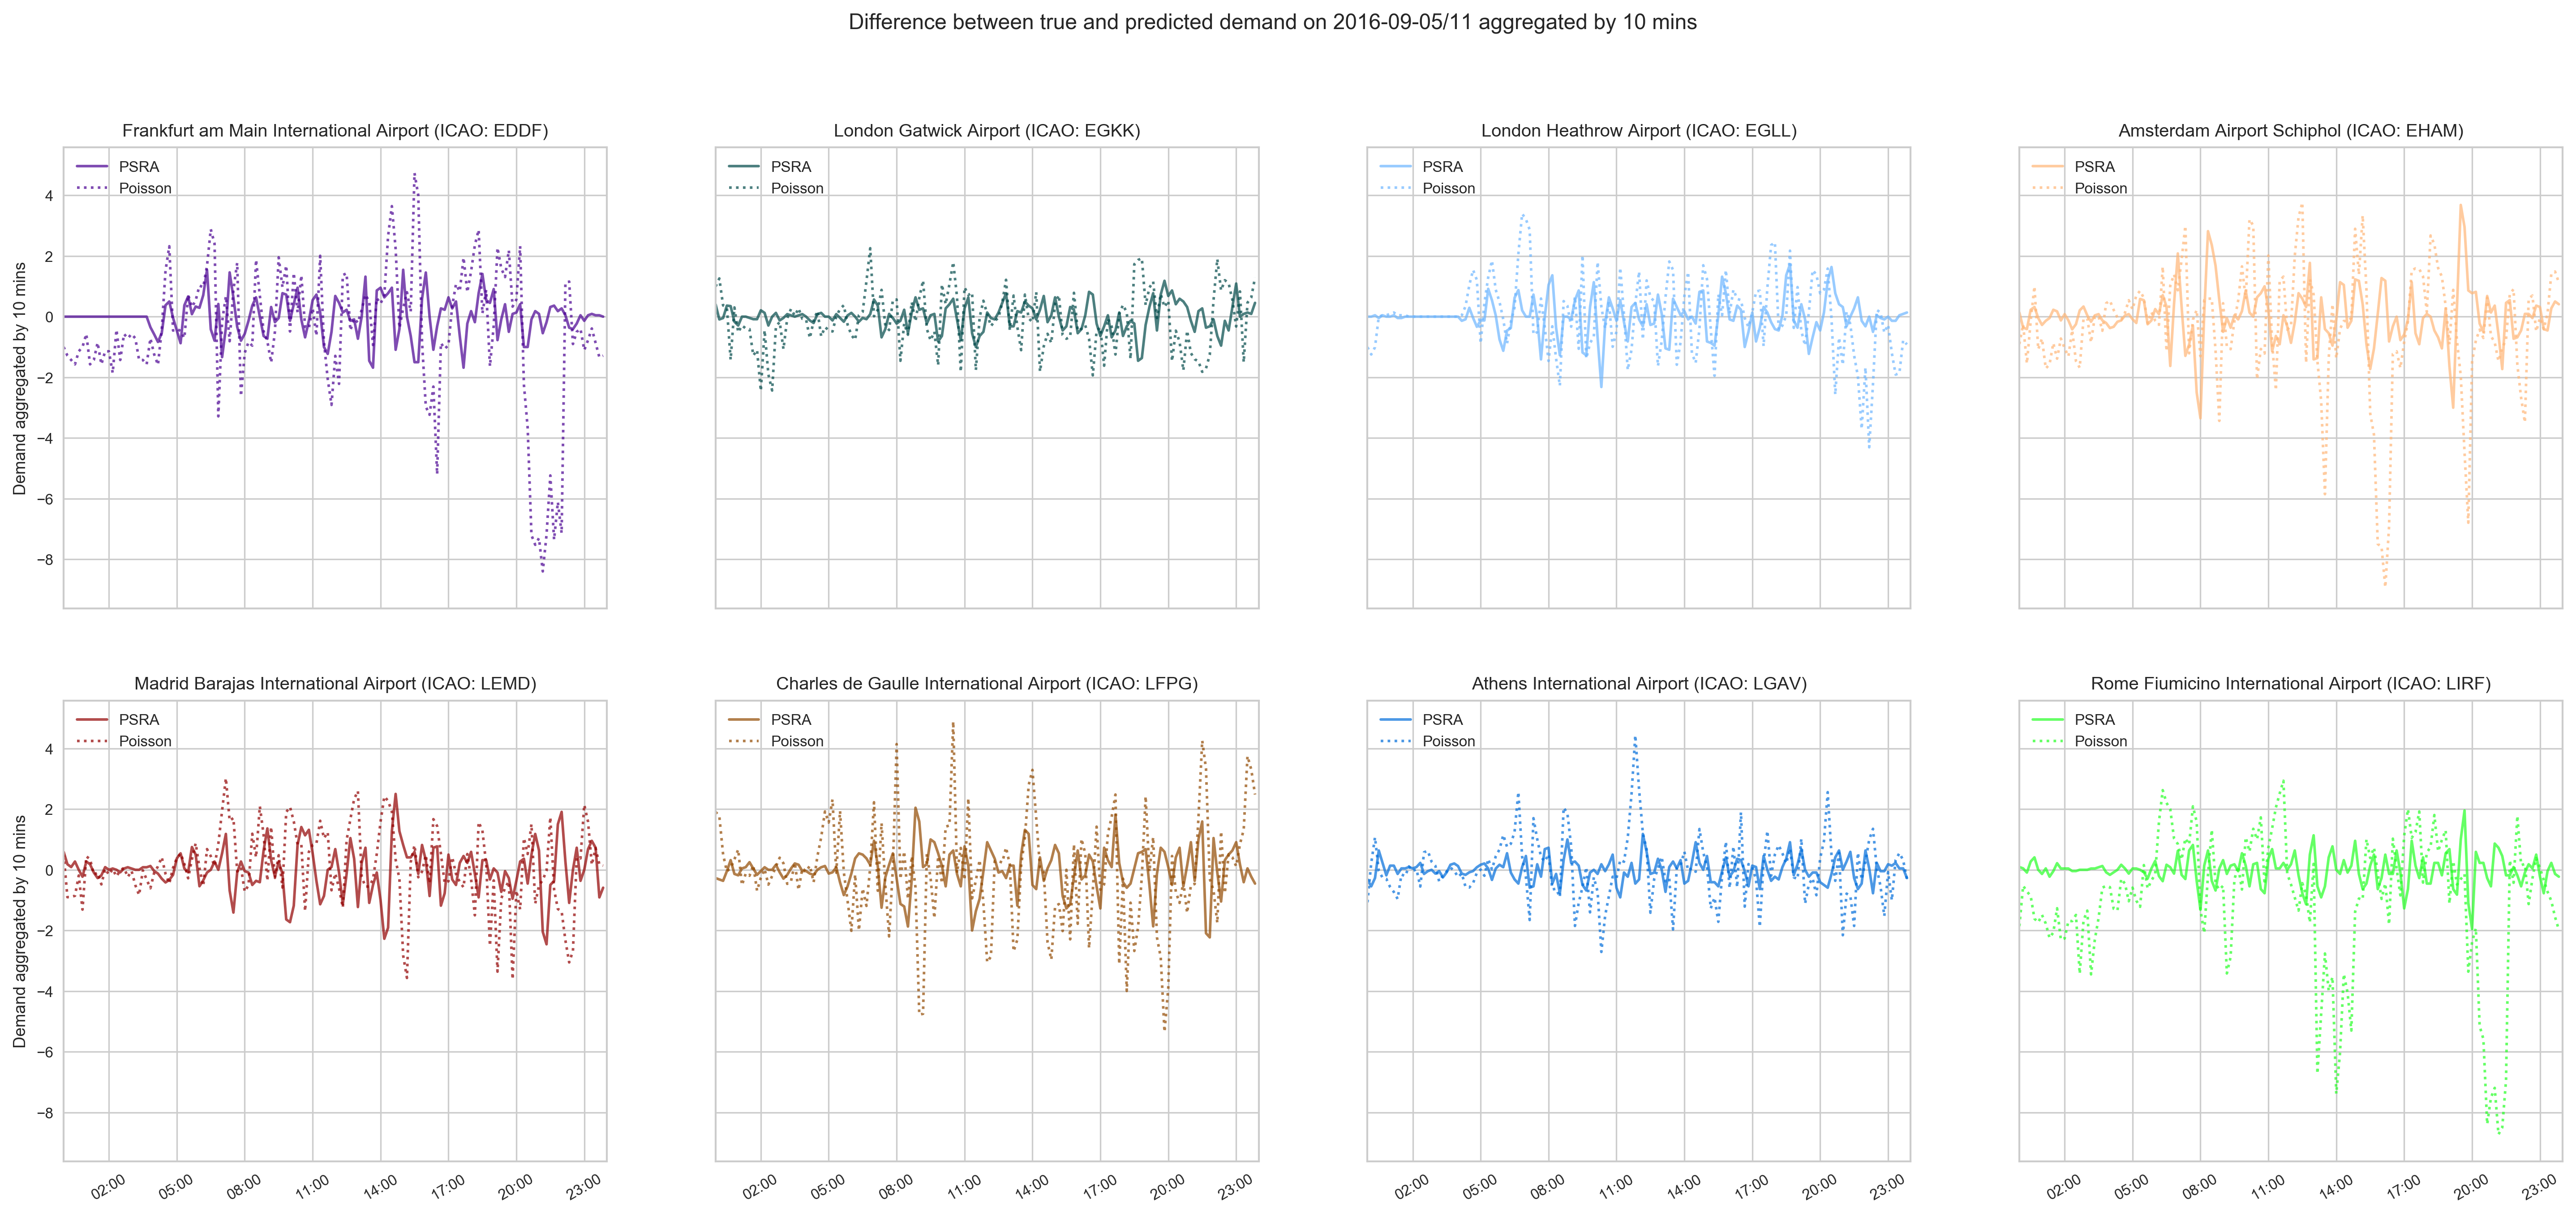
\includegraphics[width=\textwidth]{prediction_last_week}
    \caption{Difference between true and predicted average demand between September 5 and 11, 2016. A solid line shows the prediction of the \acs{PSRA} while the dotted one that of the non-homogeneous Poisson process defined by Table~\ref{A-tab:poisson_segmentation}.}
    \label{fig:pred_last_week}
\end{sidewaysfigure}

\begin{table}
  \centering
  \caption{Scores of prediction tasks for \acs{PSRA} and non-homogeneous Poisson model. True and predicted aggregated demand, averaged in the week September 5-11, 2016, are compared using the following scores: \acl{MAE} (\acs{MAE}), \acl{MSE} (\acs{MSE}), and \(r^2\).}
  \label{tab:predictions_last_week}
  \begin{tabular}{lllrrr}
    \toprule
    airport    & prediction & model & \acs{MAE} & \acs{MSE} & \(r^2\)  \\
    \midrule
    \airp{fra} & Sep 5-11  & \acs{PSRA} &  0.451 &   0.398 &  0.964 \\
         &                  & Poisson    &  1.624 &   5.199 &  0.531 \\
    \airp{lgw} & Sep 5-11  & \acs{PSRA} &  0.320 &   0.187 &  0.920 \\
         &                  & Poisson    &  0.748 &   0.928 &  0.602 \\
    \airp{lhr} & Sep 5-11  & \acs{PSRA} &  0.395 &   0.355 &  0.957 \\
         &                  & Poisson    &  0.959 &   1.661 &  0.798 \\
    \airp{ams} & Sep 5-11  & \acs{PSRA} &  0.629 &   0.875 &  0.921 \\
         &                  & Poisson    &  1.262 &   3.635 &  0.672 \\
    \airp{mad} & Sep 5-11  & \acs{PSRA} &  0.555 &   0.593 &  0.894 \\
         &                  & Poisson    &  0.876 &   1.491 &  0.733 \\
    \airp{cgd} & Sep 5-11  & \acs{PSRA} &  0.520 &   0.516 &  0.932 \\
         &                  & Poisson    &  1.199 &   2.764 &  0.635 \\
    \airp{ath} & Sep 5-11  & \acs{PSRA} &  0.289 &   0.143 &  0.906 \\
         &                  & Poisson    &  0.704 &   0.869 &  0.427 \\
    \airp{fco} & Sep 5-11  & \acs{PSRA} &  0.354 &   0.252 &  0.956 \\
         &                  & Poisson    &  1.668 &   6.104 & -0.064 \\
    \bottomrule
  \end{tabular}
\end{table}

\begin{sidewaysfigure}
    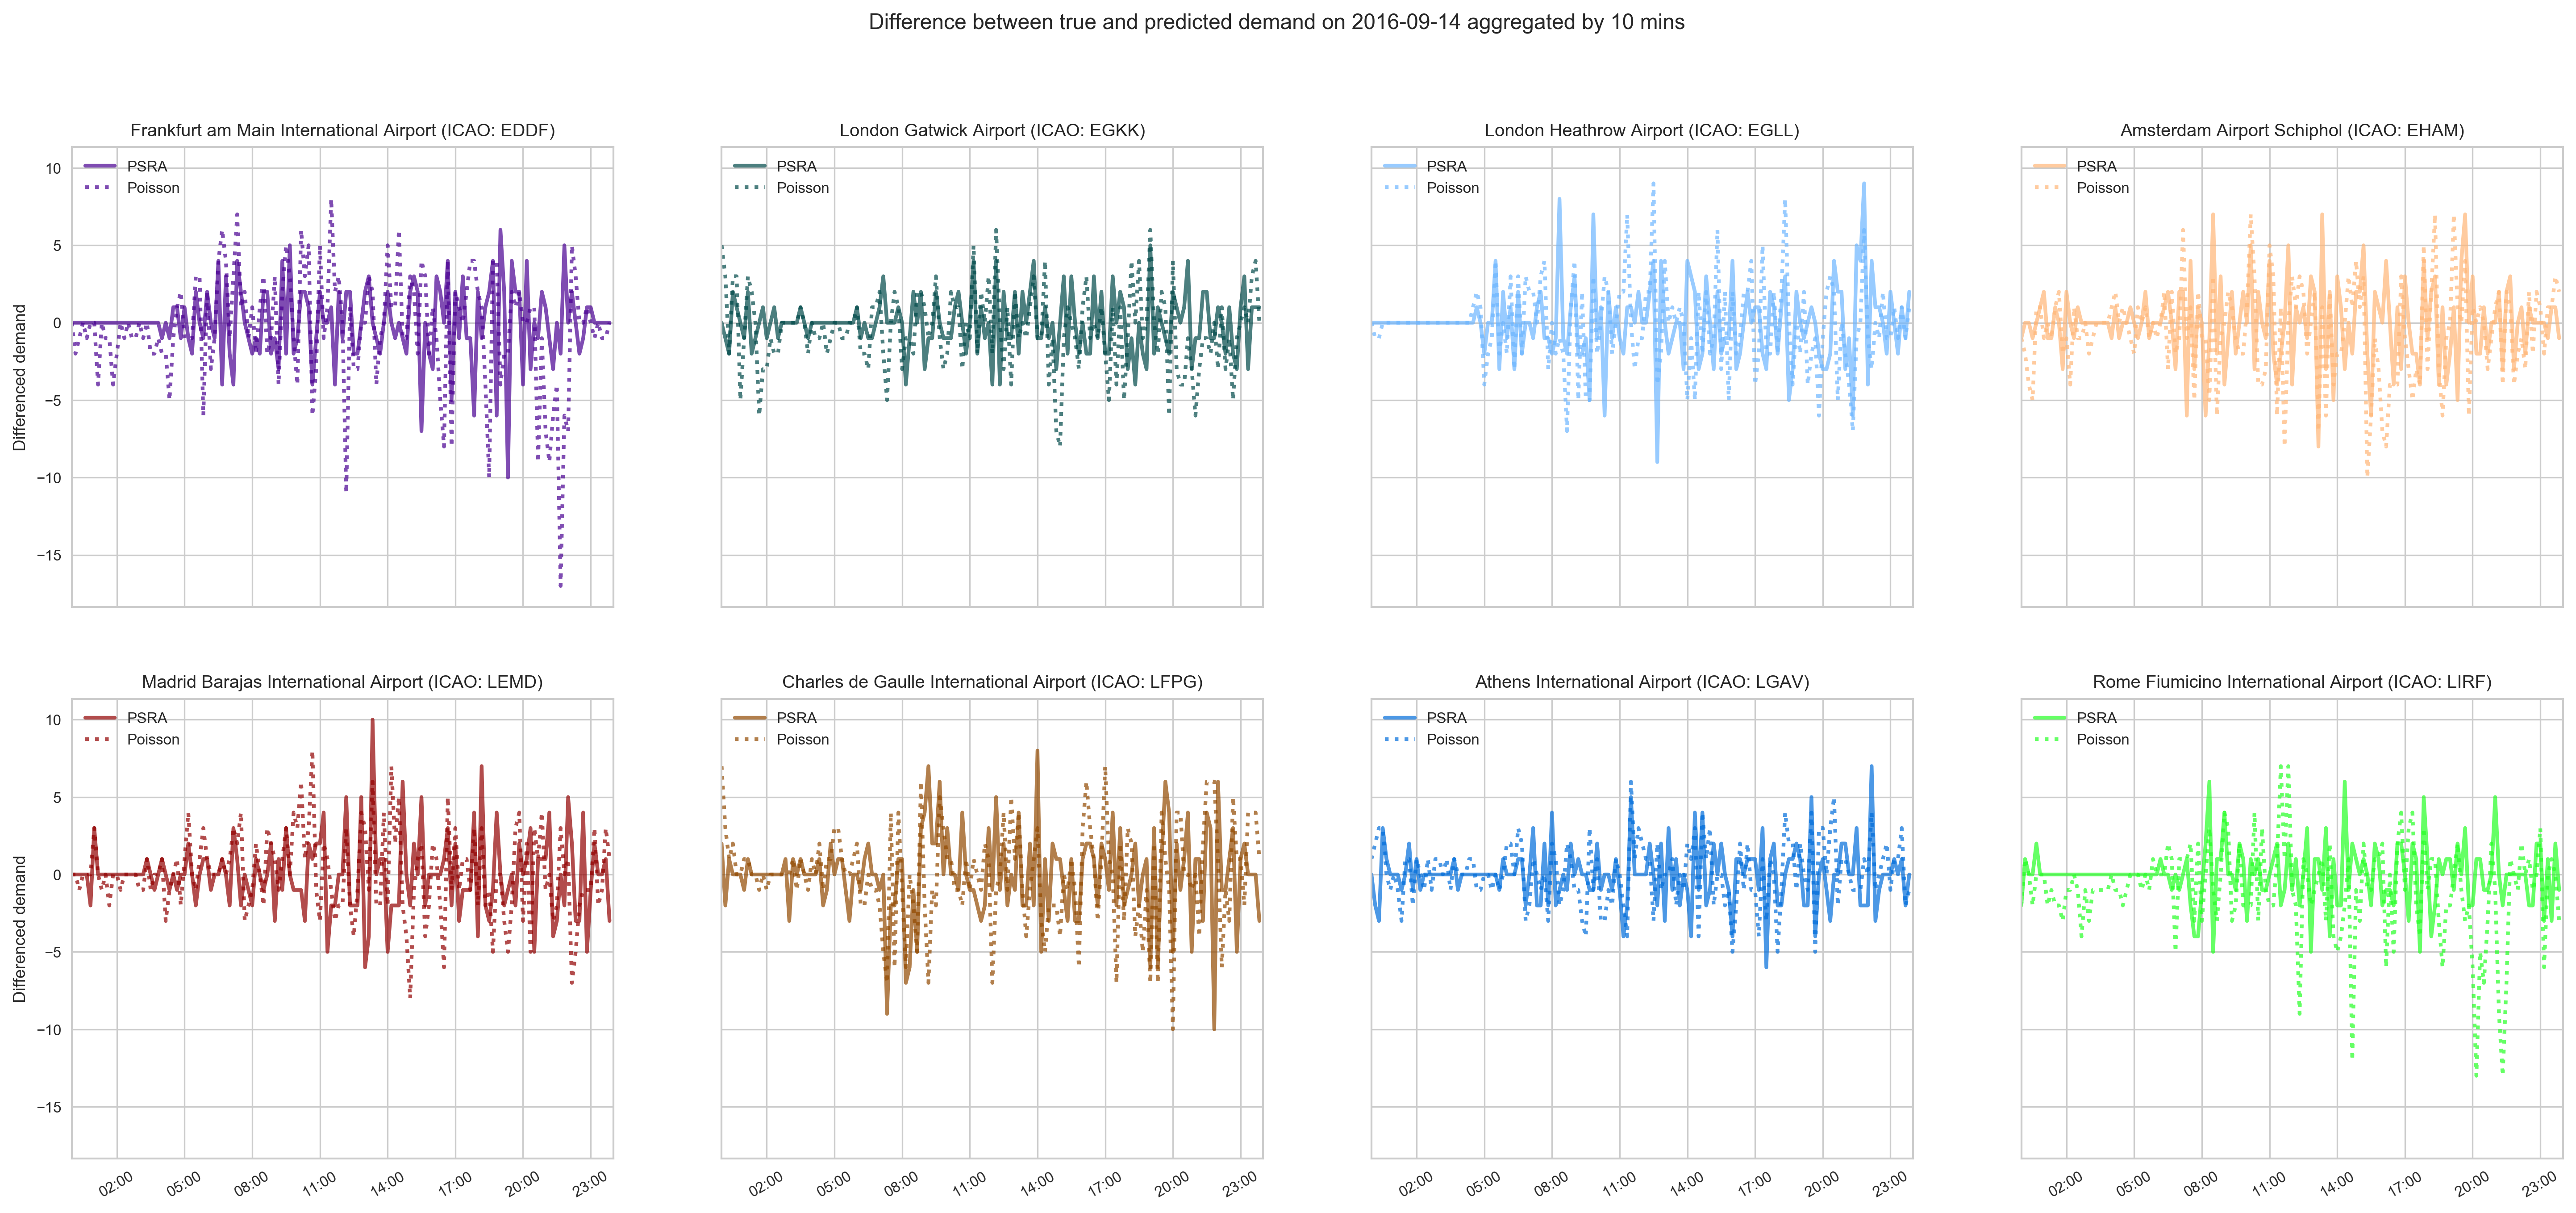
\includegraphics[width=\textwidth]{prediction_last_day}
    \caption{Difference between true and predicted demand on September 14, 2016. A solid line shows the prediction of the \acs{PSRA} model while the dotted one that of the non-homogeneous Poisson process defined by Table~\ref{A-tab:poisson_segmentation}.}\label{fig:pred_last_day}
\end{sidewaysfigure}

\begin{table}
  \centering
  \caption{Scores of prediction tasks for \acs{PSRA} and non-homogeneous Poisson model. True and predicted aggregated demand on September 14, 2016 are compared using the following scores: \acl{MAE} (\acs{MAE}), \acl{MSE} (\acs{MSE}), and \(r^2\).}\label{tab:predictions_last_day}
  \begin{tabular}{lllrrr}
    \toprule
    airport    & prediction & model & \acs{MAE} & \acs{MSE} & \(r^2\)  \\
    \midrule
    \airp{fra} & Sep 14    & \acs{PSRA} &  1.611 &   5.472 &  0.597 \\
         &                  & Poisson    &  2.597 &  11.972 &  0.119 \\
    \airp{lgw} & Sep 14    & \acs{PSRA} &  1.292 &   3.069 &  0.286 \\
         &                  & Poisson    &  1.660 &   5.174 & -0.203 \\
    \airp{lhr} & Sep 14    & \acs{PSRA} &  1.646 &   5.979 &  0.427 \\
         &                  & Poisson    &  1.944 &   8.236 &  0.211 \\
    \airp{ams} & Sep 14    & \acs{PSRA} &  1.826 &   6.493 &  0.541 \\
         &                  & Poisson    &  2.375 &  10.347 &  0.268 \\
    \airp{mad} & Sep 14    & \acs{PSRA} &  1.618 &   5.688 &  0.332 \\
         &                  & Poisson    &  2.042 &   8.611 & -0.012 \\
    \airp{cgd} & Sep 14    & \acs{PSRA} &  1.958 &   7.778 &  0.170 \\
         &                  & Poisson    &  2.785 &  13.813 & -0.475 \\
    \airp{ath} & Sep 14    & \acs{PSRA} &  1.243 &   3.396 & -0.072 \\
         &                  & Poisson    &  1.549 &   4.771 & -0.506 \\
    \airp{fco} & Sep 14    & \acs{PSRA} &  1.222 &   3.444 &  0.561 \\
         &                  & Poisson    &  2.222 &   9.097 & -0.159 \\
    \bottomrule
  \end{tabular}
\end{table}

\section{Analysis}\label{sec:analysis}

  Analysis of inter-arrival times at 40 NM showed a fair accordance between data and a Weibull distribution; this was already known in the literature for \emph{projected} inter-arrivals at some major US airports~\citep{willemain2004statistical}.
  The shape parameter of the fitted Weibull was sufficiently close to unity to seemingly justify the \emph{classical} assumption of Poisson arrivals\footnote{Necessary and sufficient condition for a random process to be Poisson is that inter-arrival times are \emph{independent} and exponentially distributed.}.
  The null hypothesis of Weibull-distributed \ac{IID} inter-arrivals could often be rejected based on the Kolmogorov-Smirnov goodness-of-fit test, yet this finding requires caution: due to the large sample size, the test is extremely powerful (especially at the most congested airports) and likely to flag even small deviations of the empirical distribution from the theoretical one.
  The average demand plotted in Figure~\ref{fig:AvgArrivals} suggests that the goodness-of-fit might be related to the wavy variation of the demand.
  On the one hand, QQ-plots in Figures~\ref{fig:qqplot5-8}-\ref{fig:qqplot5-17} show that the best fit is achieved by airports where the demand is stable over time, \eg{} \airp{lgw} or \airp{lhr}.
  On the other hand, the selected time windows often span moments of lower and higher demand, so that a better fit might be probably obtained by letting $\beta$, the shape parameter in~\eqref{eq:DWeibullPMF} vary over time.
  Yet, the analysis of the demand correlations in Figure 6 indicates that a non-homogeneous Poisson process is not realistic anyway due to the independence of its increments. In fact, the demand over two consecutive intervals is characterized by non-zero correlations (point estimates mostly negative and often significant at the 5\% level), which in contrast with the assumption of independent increments.

  Homogeneous or not, Poisson processes remain a popular choice for modeling inbound air traffic~\citep{gwiggner2014data}.
  Thus, we proposed a novel data-driven approach to the modeling of a non-homogeneous Poisson process by use of \PELT{} (a change-point detection algorithm) and \DBSCAN{} (clustering).
  Poisson arrivals defined this way were contrasted with a \ac{PSRA} point process, where the observed arrival time arises as the sum of the last-agreed arrival time and a random fluctuation.
  A parametric distribution is the typical modeling solution for the the delays \(\xi_i\) in~\eqref{eq:psra-like}, but we introduced an element of novelty by adopting also for \ac{PSRA} a data-driven approach.
  We used a support vector machine but other choices, like ordinary/generalized least squares or other penalized regressions, are viable options worth to be explored.

  The \ac{PSRA} model presented here could be hastily criticized on the limited number of features used.
  While it is true that a larger number of covariates could be obtained from the \ac{DDR}, recent constrains imposed to the use of such repository limited the amount of data that we could use.
  Further, the use of meteorological conditions as a predictor of delay would arguably increase the training performance of the model, but worsen its testing metrics due to the high uncertainty associated with weather forecasts.
  Yet Tables~\ref{tab:predictions_last_week} and~\ref{tab:predictions_last_day} shows that, \ac{PSRA} often score a \(r^2\) much larger than 0 even with a small number of features, indicating that a substantial part of demand variance is already captured by the model.
  \emph{On the premise that the predictive power of such formulation of \ac{PSRA} could only increase if a larger number of features were used, this work validated the idea that \ac{PSRA} are preferable over a Poisson model for modeling inbound air traffic.}

  The predictive accuracy of \ac{PSRA} over the Poisson process is demonstrated by Figures~\ref{fig:pred_last_week} and~\ref{fig:pred_last_day}, where Poisson arrivals show a larger fluctuation of the predicted demand around the true value.
  As a consequence, using such arrival process in a queue model would lead to overestimating the congestion.
  As reported by~\citet{caccavale2014model}, such overestimation can be substantial.

  One could argue that the accuracy of the Poisson process could be increased by modeling the intensity of the process on a finer time scale, \ie{} by estimating it in small prescribed intervals --it is well known that the \ac{MLE} of the parameter \(\lambda\) is the sample mean.
  Thus, a Poisson process with \(\lambda(t)\) \emph{forced} to vary every 10 minutes would be a model that exactly reproduces the daily average aggregated demand.
  While it is not obvious that such highly-parametric model would score much better than the one presented here, it would still fail to capture the correlation structure of the arrival data because a non-homogeneous Poisson process has independent increments regardless of the functional form of the intensity \(\lambda(t)\).
  Conversely, our \ac{PSRA} model preserves the right correlation structure of the demand by inheriting it from the regulated flight plan, see~\ref{A-sec:appb} in the supplementary material.
  In addition, \ac{PSRA} have the general property of converging to a Poisson stream in the regime of delays with very large standard deviation~\citep{guadagni2011queueing}. In other words, PSRA can produce a stream of customers that is similar to a Poisson process but has the right correlation structure .

\section{Conclusions}\label{sec:conclusions}

  %  The paper analyses a dataset of inbound traffic data at eight important European airports. Having in mind the description of airport congestion through a queuing system, we have modeled the inbound stream of aircraft in a data-driven fashion. For simplicity, we have considered the entrance time of an idealized cylinder of radius 40 NM centered at the arrival airport. The analytical tools used and the methodological approach highlighted above would not be affected if that time was to be replaced by a the first entrance-time in a geographically-specified airspace volume.

  % This paper has presented many arguments to adopt a \ac{PSRA} point process for modeling the aircraft inbound flow. The current main limitation to the use of the \ac{PSRA} family is the great difficulty of any analytical treatment as soon as the distribution of \(\xi\) is non-trivial. However, promising results have been recently presented in~\citet{lancia2013advances} for the case of exponential \(\xi_i\)'s.

  %  All in all, the final outcome of the paper is a general recommendation of preferring, whenever possible, the adoption of \ac{PSRA} for the modeling and simulation-based analyses of the inbound traffic over any process in the family of Poisson arrivals.

  %% LAST CARLO In this paper, we offered a thorough analysis of the inbound traffic at eight European airports using a data-driven a Poisson and a \ac{PSRA} model, which we compared on their capabilities of predicting future demand. In view of the results obtained, we recommend to adopt, whenever possible, \ac{PSRA} any process in the family of Poisson arrivals for modeling and simulation-based analyses of the inbound traffic.


  In this paper, we offered a thorough analysis of inbound air traffic at eight European airports. We developed two data-driven models for the prediction of the demand, one in the family of Poisson arrivals and the other in the family of \ac{PSRA}.
  In all the considered airports, the \ac{PSRA} process provides better predictions on the arrival stream.
  The superior predictive power of the proposed \ac{PSRA} over the proposed non-homogeneous Poisson process is not a reason \emph{per se} to recommend one model or the other.
  Yet, given the correlation of the demand over consecutive intervals, it is clear than a Poisson process is not a good candidate for the description of the inbound traffic flow in Europe. Their use for the estimation of inbound congestion might result in pronounced overestimation, as discussed in the introduction; conversely, \ac{PSRA} are correlated, provide more accurate predictions, and can be viewed as a generalization of Poisson arrivals from a mathematical point of view. For all these reasons, we recommend to consider \ac{PSRA} as a modelling option because we observe that, in the European context, they are preferable from many points of view.

  The proposed approach should be envisioned in simulation-based analysis of air traffic management initiatives at either strategic or planning phase.
  More specifically, it can be used as an engine to support and assess flight schedule development and strategic slot allocation schemes.
  The analysis can target either the single airport and the implications on its operations or the ATM network and its overall performances.
  In the latter case, the proposed model will be one of the atomic components of a larger embedded simulation model.
  On a longer time horizon, the proposed model can be used to evaluate long term growth initiatives such as airport expansions.
  Several airports around the world, like London Heathrow and Rome Fiumicino in Europe, are planning to increase their capacity.
  Thus, it would be advisable to have accurate studies on the possible gains in terms of available capacity and performances of the system.

  The proposed model for inbound air traffic demand is also recommendable to fine-tune Traffic Management Initiatives on a shorter time scale such as Ground Delay Programs.
  However, in this case it might be advisable to extend the predicting models to include weather features, similarly to~\cite{liu2017} and~\cite{gopal2017}.

\clearpage

% \appendix
%
% \section{\PELT{} with \acs{MBIC} and \acs{AIC} penalty}\label{sec:appa}
%
%   This appendix offers a sensitivity analysis of the \PELT{} algorithm with respect to the result of Algorithm~\ref{Alg:POISSON}.
%   Figure~\ref{fig:DD_MBIC} shows the change-point identified by \PELT{} and the resulting clustering via \DBSCAN{} when \PELT{} uses the default \ac{MBIC} penalty.
%   In this case, the change-points returned by \PELT{} are so well-concentrated that the clustering step is barely needed.
%   Accordingly, the number of outliers returned by \DBSCAN{} (shown in black) is extremely limited.
%   Identified clusters are limited in number and typically located early in the morning or late in the evening.
%   Thus, the Poisson intensities returned by Algorithm~\ref{Alg:POISSON} have a very straightforward interpretation as day and night regimes.
%
%   \begin{figure}
%       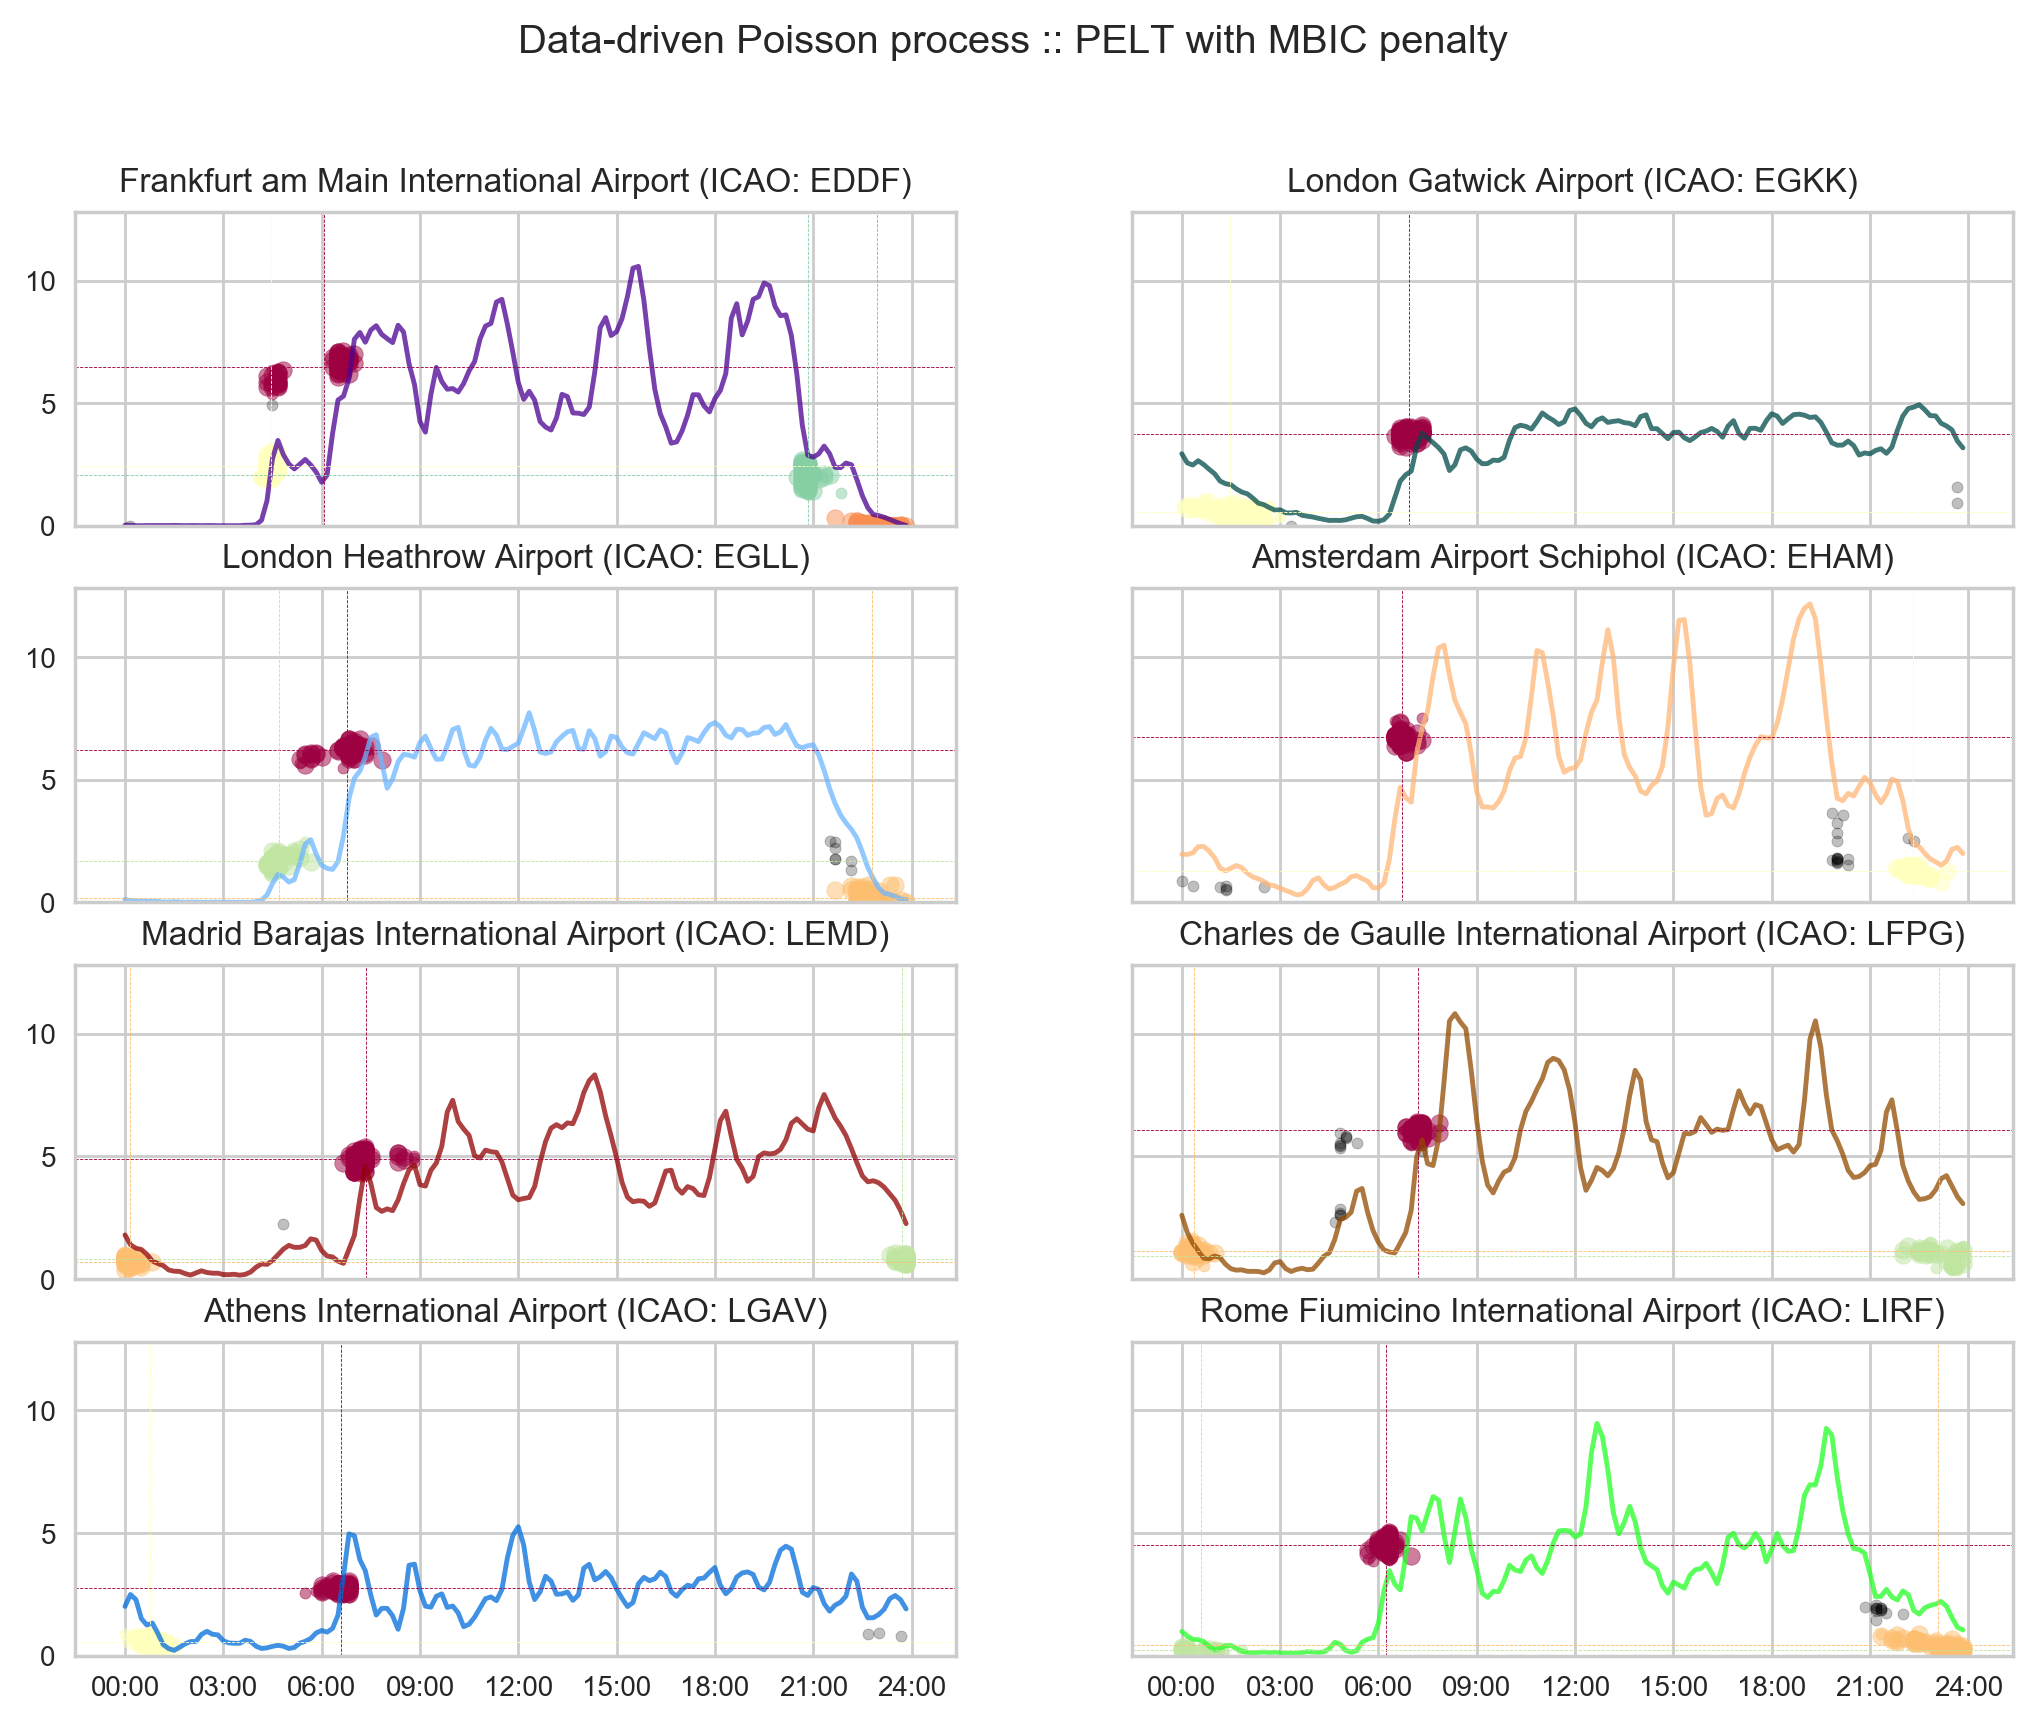
\includegraphics[width=\textwidth]{DDPoisson_MBIC}
%       \caption{Data-driven modeling of non-homogeneous Poisson process; \ac{MBIC} penalty. \DBSCAN{} outliers are drawn in black.}\label{fig:DD_MBIC}
%   \end{figure}
%
%   Figure~\ref{fig:DD_AIC} shows the change-point identified by \PELT{} and the resulting clustering via \DBSCAN{} when \PELT{} uses the \ac{AIC} penalty.
%   In this setting, \PELT{} is much more sensible and detects regime changes in correspondence of maxima and minima of the average demand.
%   The resulting description of the arrival stream in terms of a Poisson process is hence richer and follows more closely the average demand.
%   However, the increased sensibility in the change point detection comes at the price of a \emph{noisy} distribution of change-points in the \((t,\lambda)\) plane, which might be difficult to reconstruct via \DBSCAN{} (see \airp{lgw}).
%
%   \begin{figure}
%       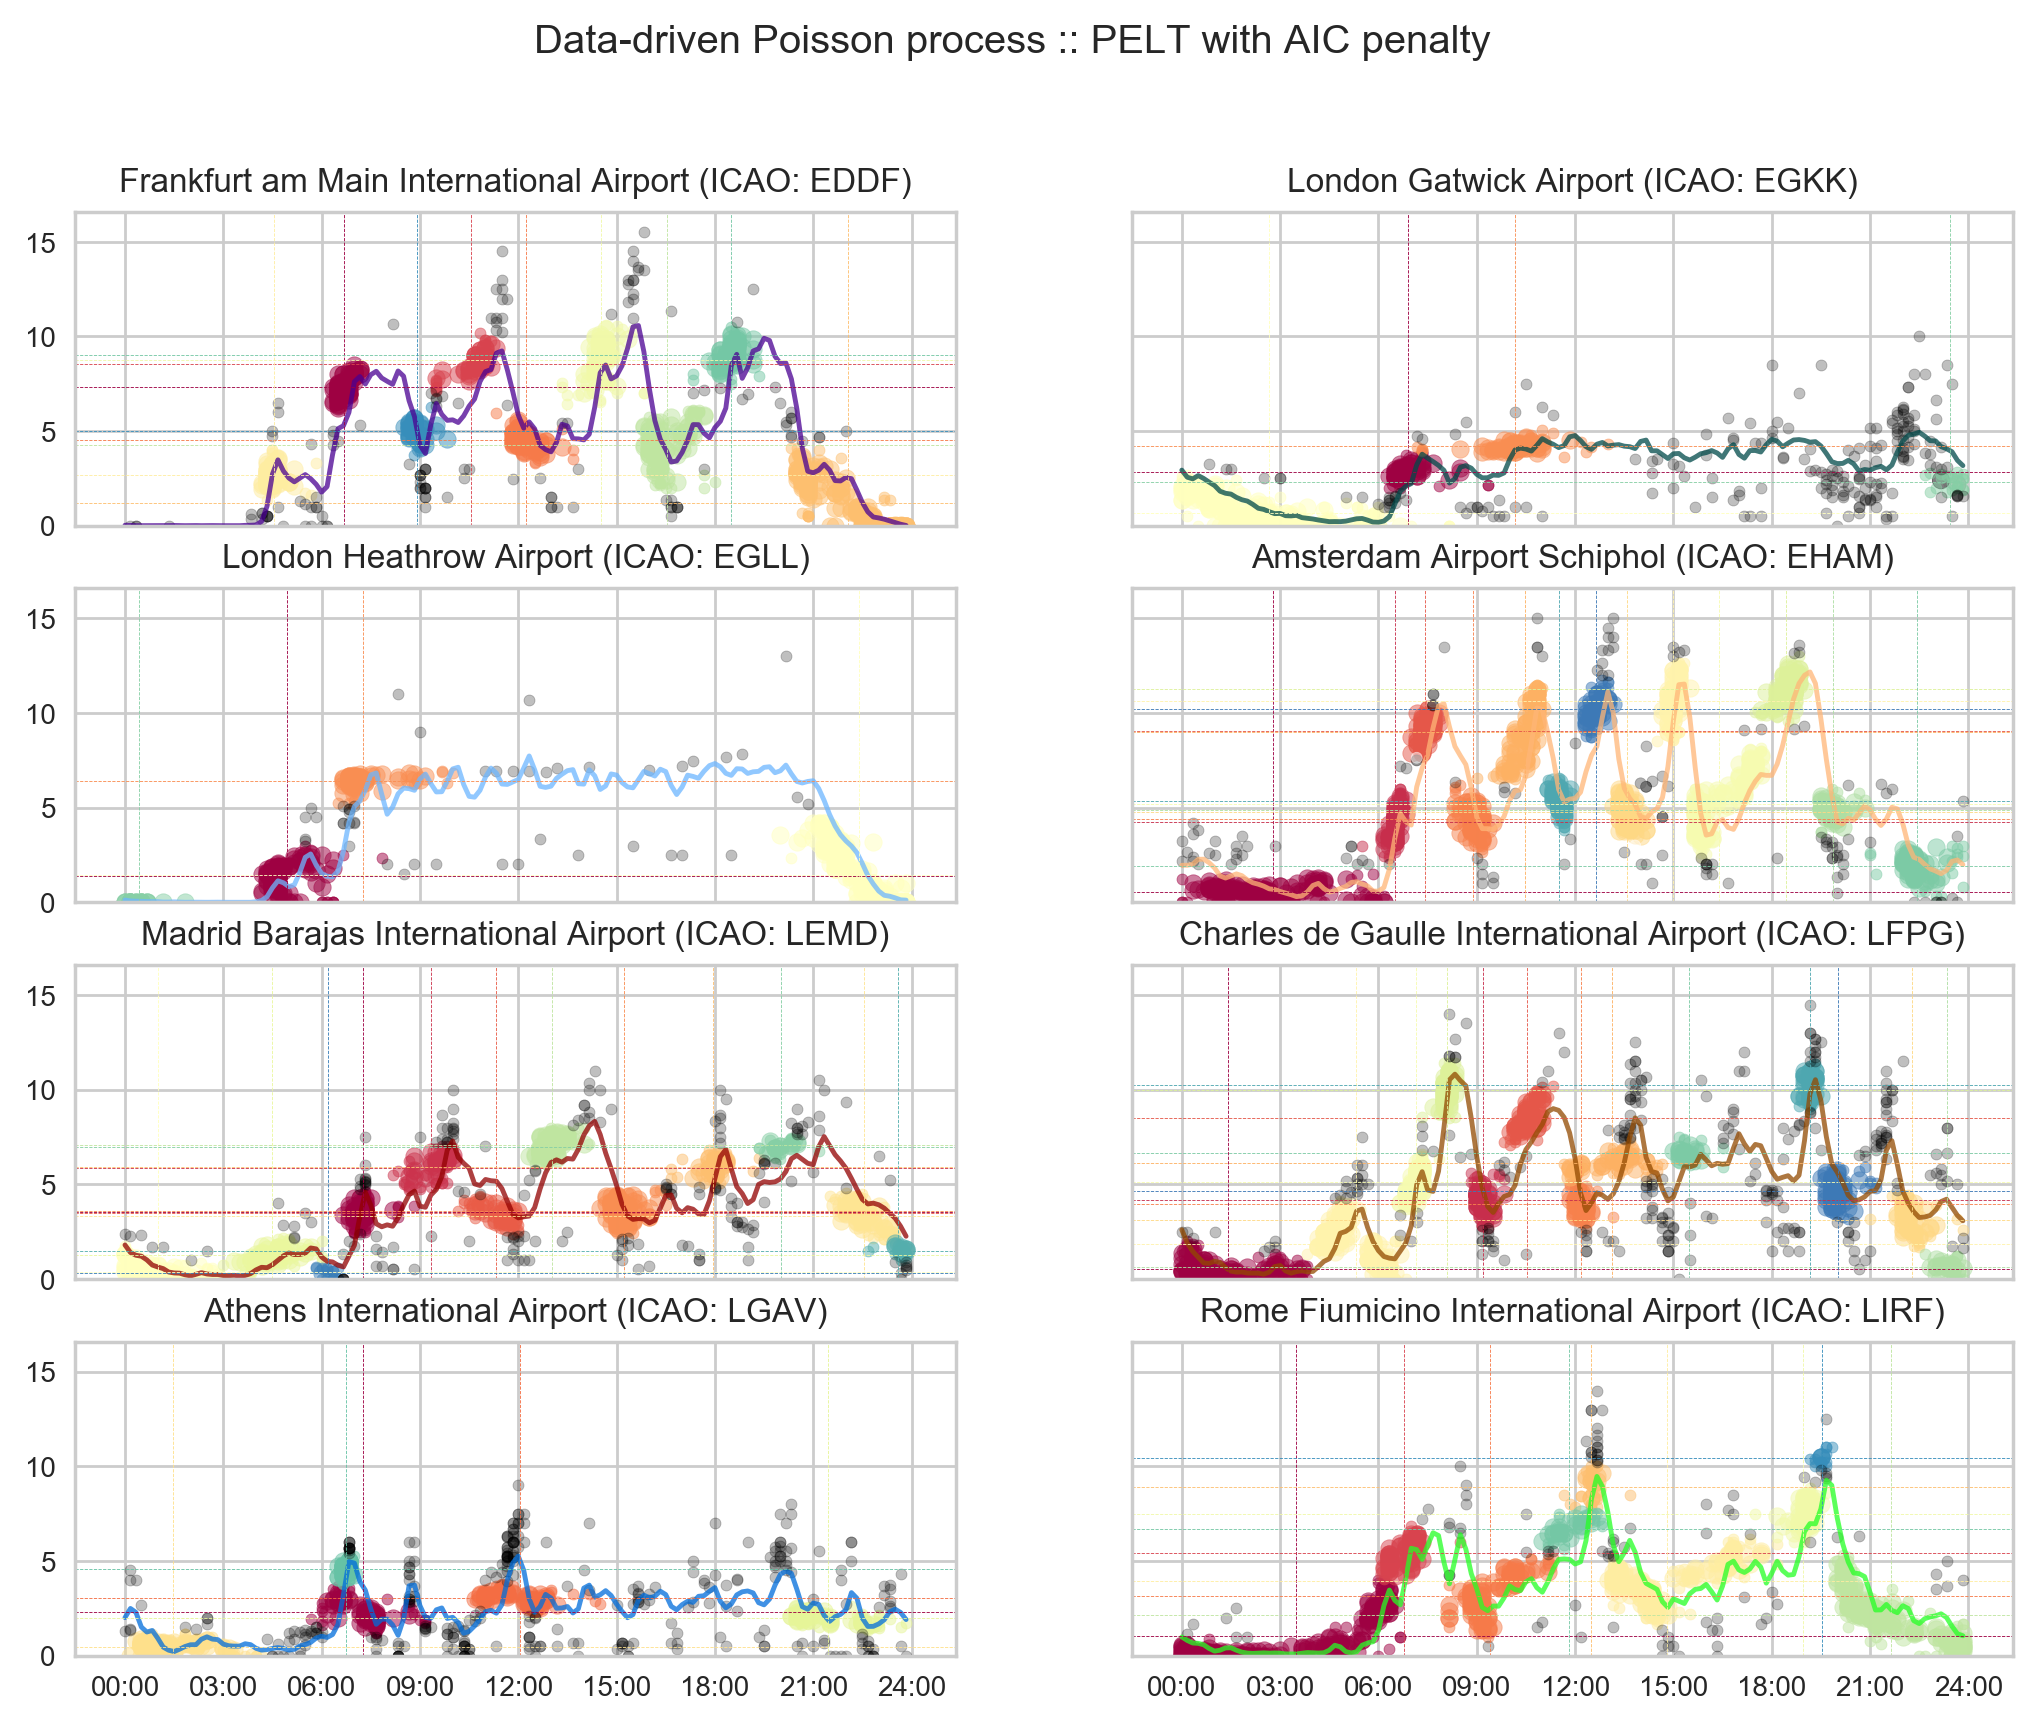
\includegraphics[width=\textwidth]{DDPoisson_AIC}
%       \caption{Data-driven modeling of non-homogeneous Poisson process; \ac{AIC} penalty. \DBSCAN{} outliers are drawn in black.}\label{fig:DD_AIC}
%   \end{figure}
%
% \section{Continuous wavelet transform of demand time series}\label{sec:appc}
%
% Figure~\ref{fig:cwt} shows a continuous wavelet transform of the demand from the week August 01--07, 2016.
% On the \(x\)-axis there is time and on the \(y\)-axis the scale parameter of the Ricker wavelet, the color bar shows the value of the coefficients of the transform. The plot highlights the presence of a low-frequency component with daily periodicity and high-frequency demand peaks with sufficient regularity, the strength and frequency of which varies across airports.
%
% % replace this with CWT
% \begin{sidewaysfigure}
%   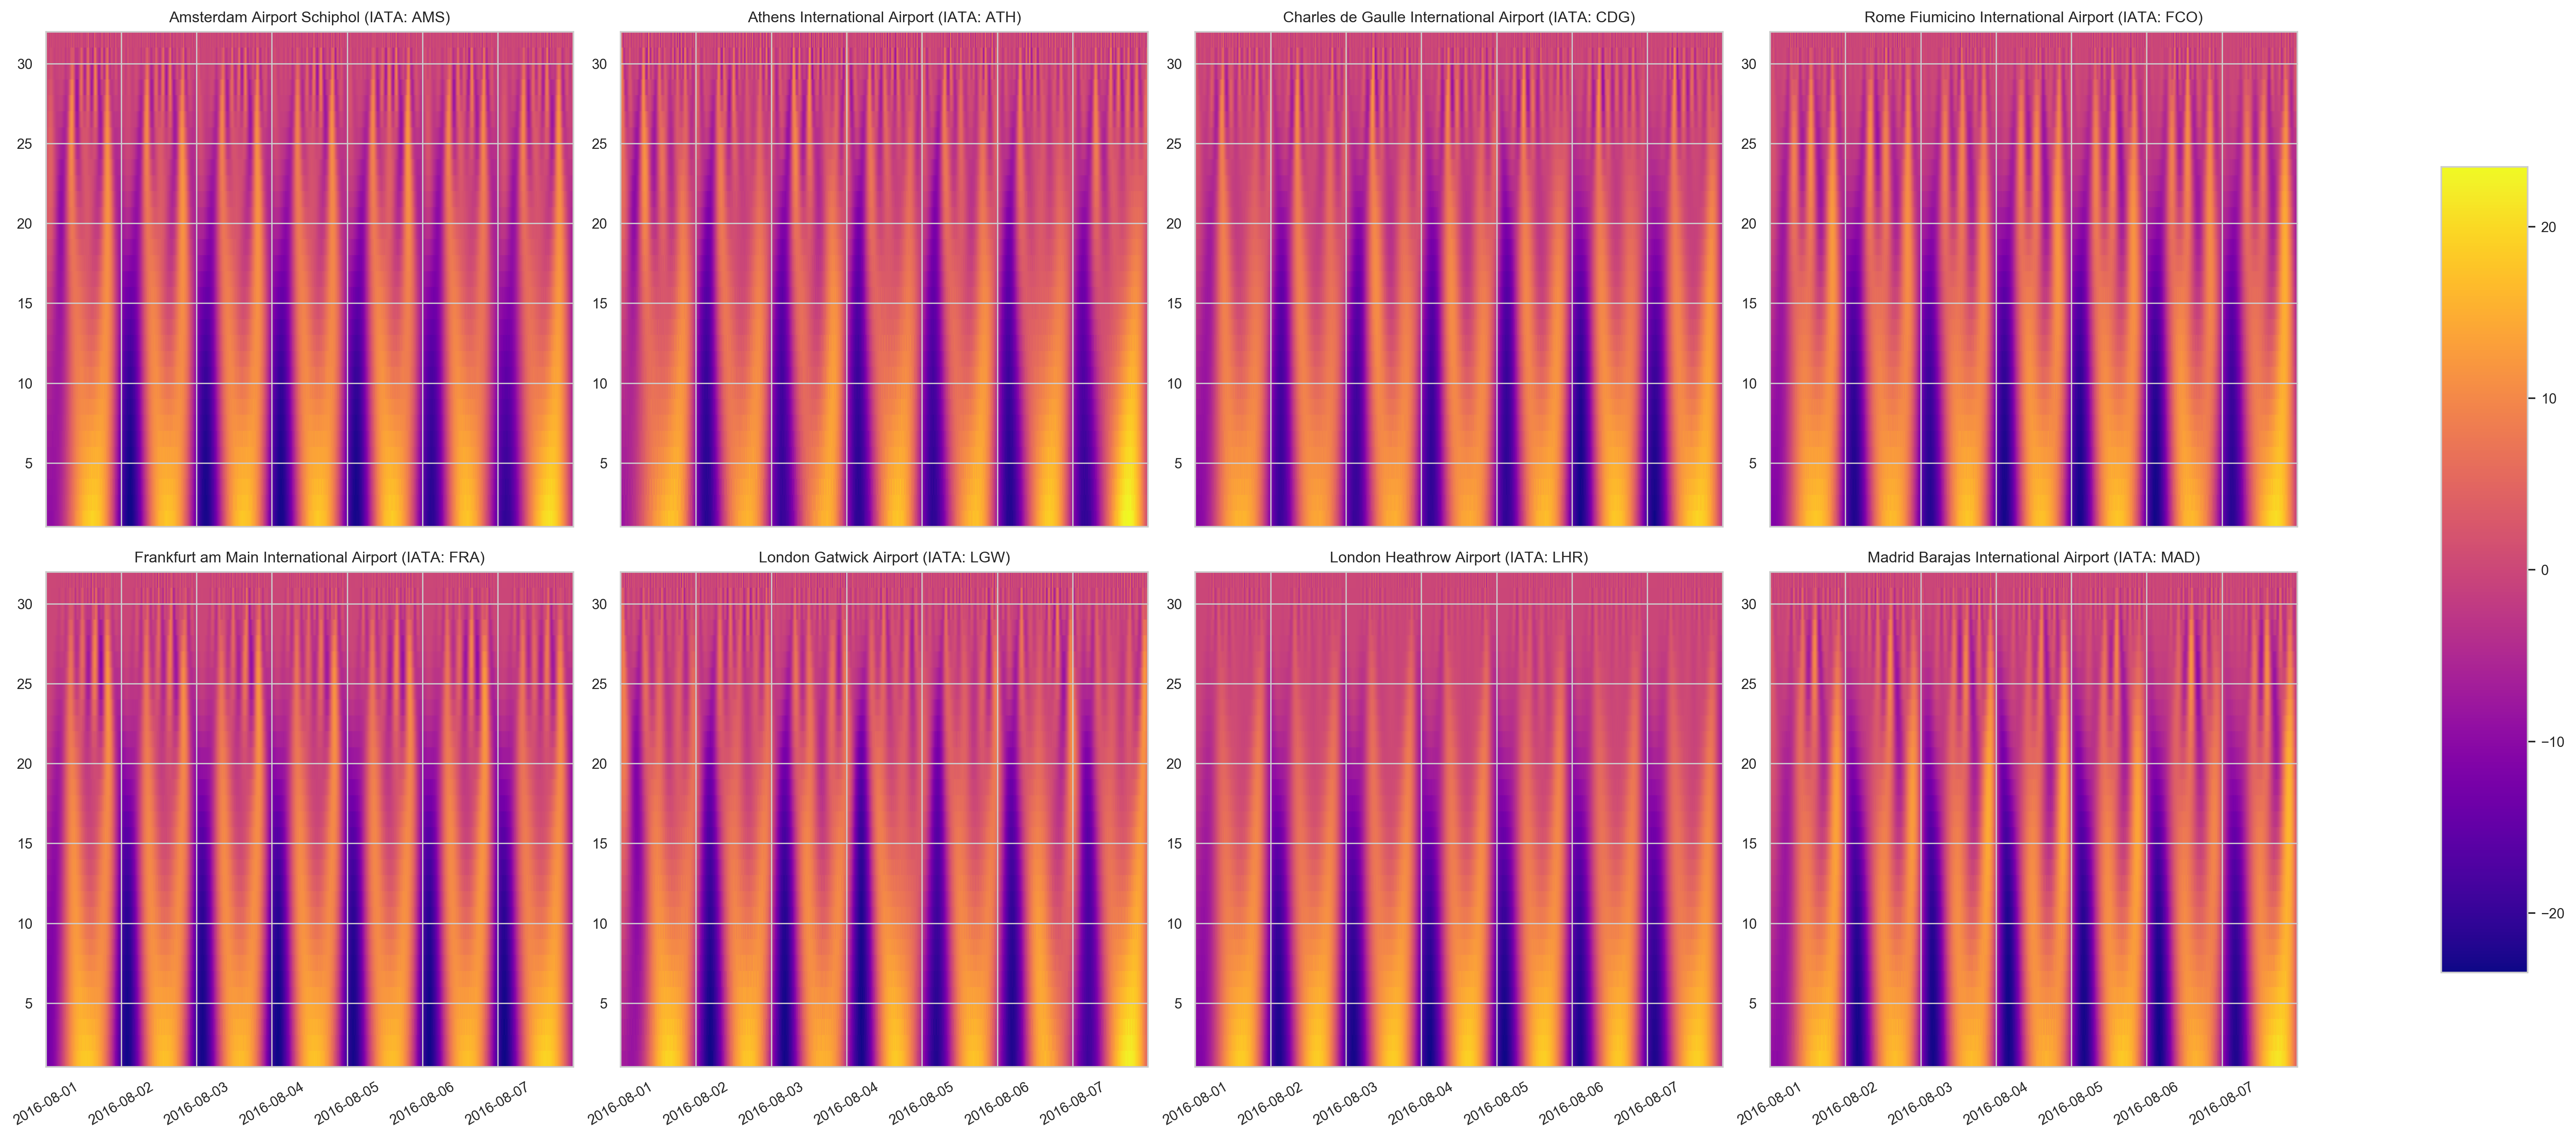
\includegraphics[width=\textwidth]{ContWavltTrasf}
%   \caption{Continuous wavelet transform of the demand for the week August 01--07, 2016. The figure clearly shows the presence of a weekly periodic component in the demand at all airport under consideration.}\label{fig:cwt}
% \end{sidewaysfigure}
%
% \section{Correlations from regulated flight plan and \acs{PSRA} model}\label{sec:appb}
%
%   Figure~\ref{fig:correlations_psra} shows the Pearson's correlation \(\rho_{t_i, t_{i+1}}\) between the simulated demand variation in the intervals \([t_i, t_{i+1})\) and \([t_{i+1}, t_{i+2})\). The simulated demand variation is obtained by subtracting the demand according to the regulated flight plan \(t^{M1}\) from the demand simulated from Model~\eqref{eq:psra-like}.
%
%   Comparing Figures~\ref{fig:correlations_true} and~\ref{fig:correlations_psra}, we observe that the \ac{PSRA} model~\eqref{eq:psra-like} captures very well this characteristic of the inbound flow.
%
%   \begin{sidewaysfigure}
%       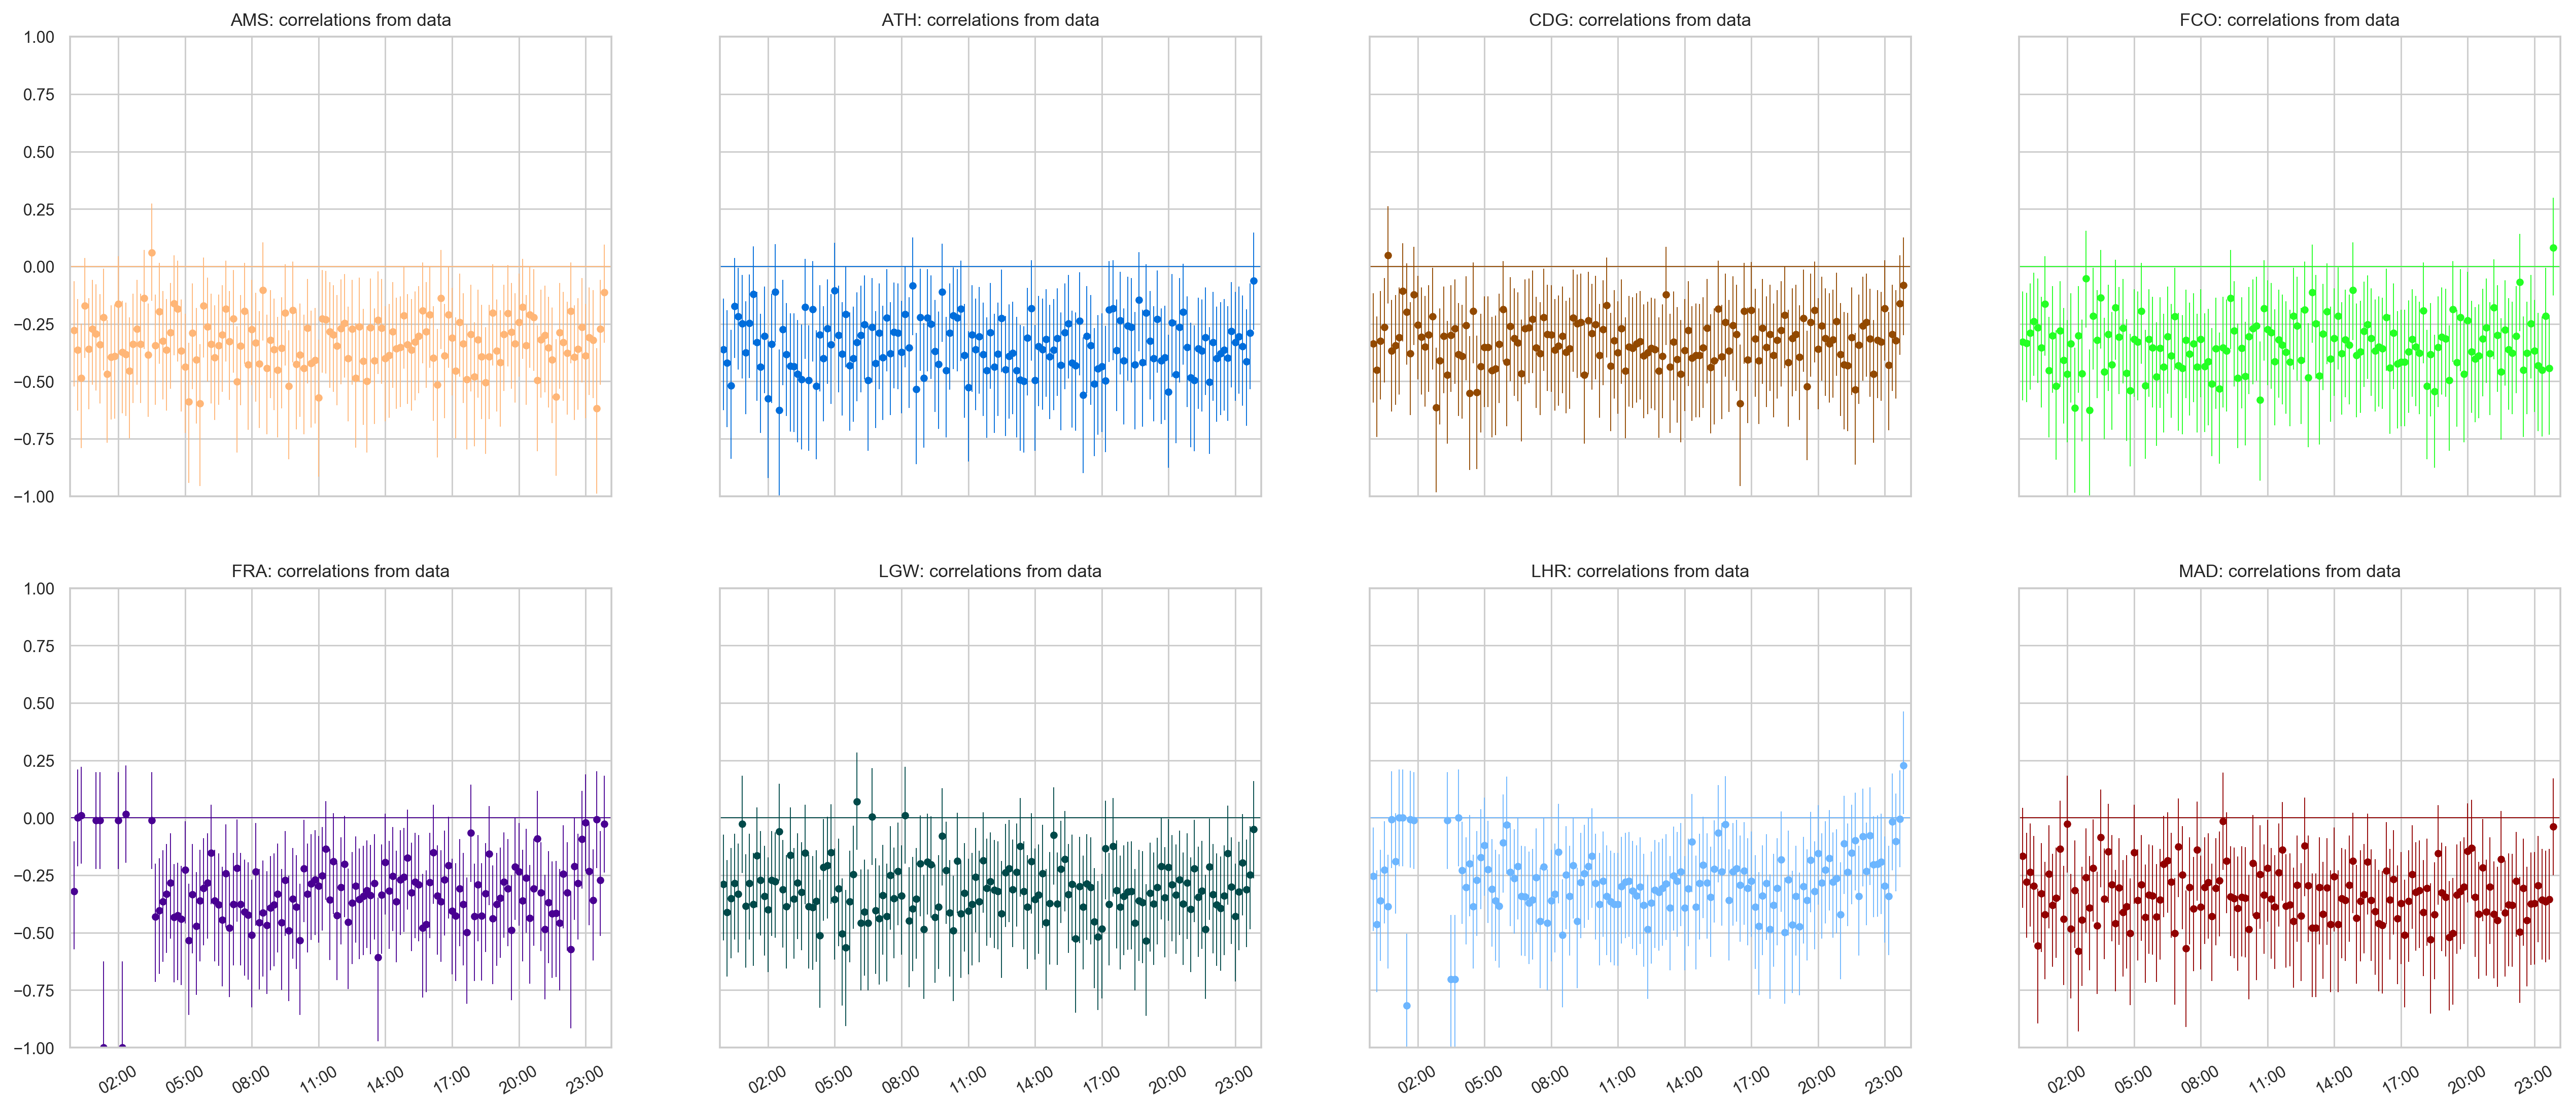
\includegraphics[width=\textwidth]{correlations_psra}
%       \caption{Correlations from simulation of Model~\eqref{eq:psra-like}. Error bars show 95\% confidence interval for Pearson's \(\rho\).}
%       \label{fig:correlations_psra}
%   \end{sidewaysfigure}
%
% % \clearpage
%
% \section{Intensity function of the data-driven Poisson process}\label{sec:appd}
%
%   This appendix details the intensity function of the Poisson process obtained in Section~\ref{sec:pois}.
%   The intensity function is a periodic right-continuous step-function, which takes on value \(\hat{\lambda}\) between two consecutive values of \(\hat{t}\).
%   The values of \(\hat{t}\) and \(\hat{\lambda}\) are reported for each airport by Table~\ref{tab:poisson_segmentation} below.
%   The table shows how the model correctly captures the typical hourly landing rate in the moments of highest demand, when we expect the airport to operate close to its maximum capacity. For \airp{lhr}, \(\lambda = 0.64\) aircraft/min corresponds to \(38.4\) aircraft/hour, which is close to the maximum declared capacity of 45; for \airp{fra}, \(\lambda = 0.90\) aircraft/min corresponds to \(54\) aircraft/hour, which is close to the maximum declared capacity of 60; finally, for \airp{ams}, \(\lambda = 1.13\) aircraft/min corresponds to \(67.8\) aircraft/hour, which is very close to the the maximum declared capacity of 68 (capacity data from \url{https://ext.eurocontrol.int/airport_corner_public/}).
%
%   \begin{center}
%     \begin{longtable}{lll}
%       \caption{Non-homogeneous Poisson process derived by \PELT{} and \DBSCAN{} algorithms. The table reports the centroids of the clusters identified by \DBSCAN{} and shown in Figure~\ref{fig:poisson_segmentation}. Times are local.}
%       \label{tab:poisson_segmentation}\\
%
%       \toprule
%       \multicolumn{1}{c}{airport} & \multicolumn{1}{c}{time} & \multicolumn{1}{c}{\(\lambda\)} \\
%       \midrule
%       \endfirsthead
%
%       \multicolumn{3}{c}%
%       {\tablename\ \thetable{} -- \emph{continued from previous page}} \\
%       \toprule
%       \multicolumn{1}{c}{airport} & \multicolumn{1}{c}{time} & \multicolumn{1}{c}{\(\lambda\)} \\
%       \midrule
%       \endhead
%
%       \midrule
%       \multicolumn{3}{r}{\emph{Continued on next page}}\\
%       \bottomrule
%       \endfoot
%
%       \bottomrule
%       \endlastfoot
%
%       \airp{fra} & 04:32 UTC+02 &  0.2657 aircraft/min \\
%            & 06:41 UTC+02 &  0.7325 aircraft/min \\
%            & 08:55 UTC+02 &  0.4991 aircraft/min \\
%            & 10:33 UTC+02 &  0.8550 aircraft/min \\
%            & 12:14 UTC+02 &  0.4530 aircraft/min \\
%            & 14:31 UTC+02 &  0.8757 aircraft/min \\
%            & 16:31 UTC+02 &  0.4270 aircraft/min \\
%            & 18:29 UTC+02 &  0.9034 aircraft/min \\
%            & 22:04 UTC+02 &  0.1182 aircraft/min \\
%       \airp{lgw} & 02:40 UTC+01 &  0.0671 aircraft/min \\
%            & 06:54 UTC+01 &  0.2858 aircraft/min \\
%            & 10:10 UTC+01 &  0.4195 aircraft/min \\
%            & 23:26 UTC+01 &  0.2328 aircraft/min \\
%       \airp{lhr} & 00:25 UTC+01 &  0.0000 aircraft/min \\
%            & 04:56 UTC+01 &  0.1409 aircraft/min \\
%            & 07:16 UTC+01 &  0.6410 aircraft/min \\
%            & 22:24 UTC+01 &  0.1424 aircraft/min \\
%       \airp{ams} & 02:47 UTC+02 &  0.0537 aircraft/min \\
%            & 06:30 UTC+02 &  0.4222 aircraft/min \\
%            & 07:25 UTC+02 &  0.9062 aircraft/min \\
%            & 08:53 UTC+02 &  0.4416 aircraft/min \\
%            & 10:28 UTC+02 &  0.9006 aircraft/min \\
%            & 11:30 UTC+02 &  0.5334 aircraft/min \\
%            & 12:38 UTC+02 &  1.0207 aircraft/min \\
%            & 13:35 UTC+02 &  0.4785 aircraft/min \\
%            & 15:00 UTC+02 &  1.0653 aircraft/min \\
%            & 16:23 UTC+02 &  0.5189 aircraft/min \\
%            & 18:26 UTC+02 &  1.1255 aircraft/min \\
%            & 19:52 UTC+02 &  0.4881 aircraft/min \\
%            & 22:26 UTC+02 &  0.1942 aircraft/min \\
%       \airp{mad} & 01:00 UTC+02 &  0.0386 aircraft/min \\
%            & 04:30 UTC+02 &  0.1240 aircraft/min \\
%            & 06:12 UTC+02 &  0.0293 aircraft/min \\
%            & 07:14 UTC+02 &  0.3511 aircraft/min \\
%            & 09:19 UTC+02 &  0.5870 aircraft/min \\
%            & 11:18 UTC+02 &  0.3470 aircraft/min \\
%            & 13:02 UTC+02 &  0.7084 aircraft/min \\
%            & 15:14 UTC+02 &  0.3574 aircraft/min \\
%            & 17:56 UTC+02 &  0.5905 aircraft/min \\
%            & 20:01 UTC+02 &  0.6972 aircraft/min \\
%            & 22:33 UTC+02 &  0.3309 aircraft/min \\
%            & 23:35 UTC+02 &  0.1493 aircraft/min \\
%       \airp{cgd} & 01:24 UTC+02 &  0.0530 aircraft/min \\
%            & 05:18 UTC+02 &  0.1852 aircraft/min \\
%            & 07:08 UTC+02 &  0.5127 aircraft/min \\
%            & 08:06 UTC+02 &  1.0003 aircraft/min \\
%            & 09:11 UTC+02 &  0.4170 aircraft/min \\
%            & 10:32 UTC+02 &  0.8515 aircraft/min \\
%            & 12:11 UTC+02 &  0.3950 aircraft/min \\
%            & 13:06 UTC+02 &  0.6116 aircraft/min \\
%            & 15:29 UTC+02 &  0.6669 aircraft/min \\
%            & 19:09 UTC+02 &  1.0227 aircraft/min \\
%            & 20:01 UTC+02 &  0.4632 aircraft/min \\
%            & 22:16 UTC+02 &  0.3120 aircraft/min \\
%            & 23:21 UTC+02 &  0.0631 aircraft/min \\
%       \airp{ath} & 01:27 UTC+03 &  0.0445 aircraft/min \\
%            & 06:45 UTC+03 &  0.4592 aircraft/min \\
%            & 07:16 UTC+03 &  0.2315 aircraft/min \\
%            & 12:03 UTC+03 &  0.3028 aircraft/min \\
%            & 21:27 UTC+03 &  0.1993 aircraft/min \\
%       \airp{fco} & 03:29 UTC+02 &  0.1019 aircraft/min \\
%            & 06:47 UTC+02 &  0.5395 aircraft/min \\
%            & 09:24 UTC+02 &  0.3155 aircraft/min \\
%            & 11:49 UTC+02 &  0.6698 aircraft/min \\
%            & 12:30 UTC+02 &  0.8899 aircraft/min \\
%            & 14:48 UTC+02 &  0.3965 aircraft/min \\
%            & 18:58 UTC+02 &  0.7465 aircraft/min \\
%            & 19:31 UTC+02 &  1.0422 aircraft/min \\
%            & 21:37 UTC+02 &  0.2130 aircraft/min \\
%     \end{longtable}
%   \end{center}
%
% \clearpage

\section*{References}

\bibliography{LL}

\end{document}
